% AER E 361 Mission Report Template
% Spring 2023
% Template created by Yiqi Liang and Professor Matthew Nelson

% Document Configuration DO NOT CHANGE
\documentclass[12 pt]{report}
% --------------------LaTeX Packages---------------------------------
% The following are packages that are used in this report.
% DO NOT CHANGE ANY OF THE FOLLOWING OR YOUR REPORT WILL NOT COMPILE
% -------------------------------------------------------------------

\usepackage{hyperref}
\usepackage{parskip}
\usepackage{titlesec}
\usepackage{titling}
\usepackage{graphicx}
\usepackage{graphviz}
\usepackage[T1]{fontenc}
\usepackage{titlesec, blindtext, color} %for LessIsMore style
\usepackage{tcolorbox} %for references box
\usepackage[hmargin=1in,vmargin=1in]{geometry} % use 1 inch margins
\usepackage{float}
\usepackage{tikz}
\usepackage{svg} % Allows for SVG Vector graphics
\usepackage{textcomp, gensymb} %for degree symbol
\hypersetup{
	colorlinks=true,
	linkcolor=blue,
	urlcolor=cyan,
}
\usepackage{biblatex}
\addbibresource{main.bib}
\usepackage{amsmath}
\usepackage{listings}
\usepackage{multicol}
\usepackage{array}

\usepackage{hologo} %KYR: for \BibTeX
%\usepackage{algpseudocode}
%\usepackage{algorithm}
% This configures items for code listings in the document
\usepackage{xcolor}

\usepackage{fancyhdr} % Headers/Footers
\usepackage{siunitx} % SI units
\usepackage{csquotes} % Display Quote
\usepackage{microtype} % Better line breaks
\usepackage{booktabs} % Better tables

\definecolor{commentsColor}{rgb}{0.497495, 0.497587, 0.497464}
\definecolor{keywordsColor}{rgb}{0.000000, 0.000000, 0.635294}
\definecolor{stringColor}{rgb}{0.558215, 0.000000, 0.135316}
\definecolor{mygreen}{rgb}{0,0.6,0}
\definecolor{mygray}{rgb}{0.5,0.5,0.5}
\definecolor{mymauve}{rgb}{0.58,0,0.82}

\lstdefinestyle{customc}{
  belowcaptionskip=1\baselineskip,
  breaklines=true,
  frame=L,
  xleftmargin=\parindent,
  language=C,
  showstringspaces=false,
  basicstyle=\footnotesize\ttfamily,
  keywordstyle=\bfseries\color{green!40!black},
  commentstyle=\itshape\color{purple!40!black},
  identifierstyle=\color{blue},
  stringstyle=\color{orange},
 }

 \lstset{ %
  backgroundcolor=\color{white},   % choose the background color; you must add \usepackage{color} or \usepackage{xcolor}
  basicstyle=\footnotesize,        % the size of the fonts that are used for the code
  breakatwhitespace=false,         % sets if automatic breaks should only happen at whitespace
  breaklines=true,                 % sets automatic line breaking
  captionpos=b,                    % sets the caption-position to bottom
  commentstyle=\color{commentsColor}\textit,    % comment style
  deletekeywords={...},            % if you want to delete keywords from the given language
  escapeinside={\%*}{*)},          % if you want to add LaTeX within your code
  extendedchars=true,              % lets you use non-ASCII characters; for 8-bits encodings only, does not work with UTF-8
  frame=tb,	                   	   % adds a frame around the code
  keepspaces=true,                 % keeps spaces in text, useful for keeping indentation of code (possibly needs columns=flexible)
  keywordstyle=\color{keywordsColor}\bfseries,       % keyword style
  language=Python,                 % the language of the code (can be overrided per snippet)
  otherkeywords={*,...},           % if you want to add more keywords to the set
  numbers=left,                    % where to put the line-numbers; possible values are (none, left, right)
  numbersep=8pt,                   % how far the line-numbers are from the code
  numberstyle=\tiny\color{commentsColor}, % the style that is used for the line-numbers
  rulecolor=\color{black},         % if not set, the frame-color may be changed on line-breaks within not-black text (e.g. comments (green here))
  showspaces=false,                % show spaces everywhere adding particular underscores; it overrides 'showstringspaces'
  showstringspaces=false,          % underline spaces within strings only
  showtabs=false,                  % show tabs within strings adding particular underscores
  stepnumber=1,                    % the step between two line-numbers. If it's 1, each line will be numbered
  stringstyle=\color{stringColor}, % string literal style
  tabsize=2,	                   % sets default tabsize to 2 spaces
  title=\lstname,                  % show the filename of files included with \lstinputlisting; also try caption instead of title
  columns=fixed                    % Using fixed column width (for e.g. nice alignment)
}

\lstdefinestyle{customasm}{
  belowcaptionskip=1\baselineskip,
  frame=L,
  xleftmargin=\parindent,
  language=[x86masm]Assembler,
  basicstyle=\footnotesize\ttfamily,
  commentstyle=\itshape\color{purple!40!black},
}

\lstset{escapechar=@,style=customc}

\titlelabel{\thetitle.\quad}

% From here on out you can start editing your document
\newcommand{\subtitle}[1]{%
  \posttitle{%
    \par\end{center}
    \begin{center}\LARGE#1\end{center}
    \vskip0.5em}%
}

\title{\textbf{Iowa State University
\\{\Large Aerospace Engineering}}}
\subtitle{AER E 322 Lab 9\\
		  Introduction to Nondestructive Evaluation}
\author{Matthew Mehrtens, Peter Mikolitis, and Natsuki Oda}

\newcommand{\etal}{\textit{et al}., }
\newcommand{\ie}{\textit{i}.\textit{e}., }
\newcommand{\eg}{\textit{e}.\textit{g}., }

% Define the headers and footers
\setlength{\headheight}{70.63135pt}
\geometry{head=70.63135pt, includehead=true, includefoot=true}
\fancypagestyle{plain}{
	\fancyhead{}\fancyfoot{} % clears the headers/footers
	\fancyhead[L]{\textbf{AER E 322}}
	\fancyhead[C]{\textbf{Aerospace Structures Laboratory Report}\\
					 \textbf{Lab 9 Introduction to Nondestructive Evaluation}\\
					 Section 4 Group 2\\
					 Matthew Mehrtens, Peter Mikolitis, and Natsuki Oda\\
					 \today}
	\fancyhead[R]{\textbf{Spring 2023}}
	\fancyfoot[C]{\thepage}
}
\pagestyle{fancy}
\fancyhead{}\fancyfoot{} % clears the headers/footers
\fancyhead[L]{\textbf{AER E 322}}
\fancyhead[C]{\textbf{Aerospace Structures Laboratory Report}\\
			  \textbf{Lab 9 Introduction to Nondestructive Evaluation}\\
			  Section 4 Group 2\\
			  Matthew Mehrtens, Peter Mikolitis, and Natsuki Oda\\
			  \today}
\fancyhead[R]{\textbf{Spring 2023}}
\fancyfoot[C]{\thepage}

\begin{document}
\maketitle
\tableofcontents

\chapter{Pre-Lab} \label{pre-lab}
\section{Introduction} \label{introduction}
% TODO: Revise
In this lab, our group was tasked with experimenting with three different types of non-destructive testing, ultrasonic testing, tap testing, simulated ultrasonic testing, and eddy current testing. Ultrasonic testing entailed finding the diameter of a defect near the bottom side of a metal plate using the volt wave amplitude on an oscilloscope. We calculated how far away the transducer face needed to be from the sample to ensure the defect was at the desired focal length of \qty{8}{in} and moved the transducer around to find the defect. For the simulated ultrasonic testing, our group changed variables in a computer program to see how each would affect the signal-to-noise ratio (SNR) overall. Our objective was to hold the amplitude of the SNR above \num{4.5} for as long as possible. Eddy current testing was performed on two different aluminum bar samples (BKI and BKII) with different defects and defect sizes. BKI had cuts that simulated cracks of depths ranging from \qtyrange{0.5}{1.5}{\mm}, whereas BKII had four machined slots, which reduced the thickness of the material to \qtylist{2;1.6;1.2;0.8}{\mm}. We also utilized eddy current testing to sort small metal samples based on the trace left from coming into contact with each sample. Finally, our group used tap testing to test a plate with three defects (delamination, unbonds, and crushed cores). We then observed the tap duration while tapping each defect area to see which defects provided the longest tap duration. The overall purpose of this lab was to introduce our group to non-destructive testing to see in what scenarios each form of testing was most effective. With this, this lab helped demonstrate how non-destructive testing can be a cost-efficient, effective way to test the longevity of a part in question.

\section{Objectives} \label{objectives}
% TODO: Revise
\textbf{Ultrasonic Testing} 
\begin{itemize}
	\item Accurately predict the diameter of the defect.
	\item Get familiar with Tektronix TDS 200B oscilloscope.
	\item Correctly calculate the distance the transducer needs to be from the top face of the metal sample.
\end{itemize}

\textbf{Simulated Ultrasonic Testing}
\begin{itemize}
	\item Observe what settings affect the depth profile the most, \ie transducer type, transducer diameter, focal length, center frequency, bandwidth, and water path.
	\item Get the signal-to-noise ratio to maintain above \num{4.5} for as long as possible for each hole location.
\end{itemize}     

\textbf{Eddy Current Testing}
\begin{itemize}
	\item Observe how different metal types will leave varied traces while coming into contact.
	\item Observe where each crack is located in both the BKI and BKII samples.
	\item Adjust the frequency for each testing scenario to ensure the best results.
\end{itemize}

\textbf{Tap Testing}
\begin{itemize}
	\item Observe how each type of defect affects the data.
	\item Observe how to size of the defect area affects the data.
	\item See how different defects affect the effectiveness of tap testing.
\end{itemize}

\section{Hypothesis} \label{hypothesis}
\textbf{Ultrasonic Testing}

During the ultrasonic testing portion of the lab, we predict we will be able to locate the flaw by using the sequential search method where we first locate the transducer signal, then the front surface, then the back surface, and finally the flaw---which should be located just before the back surface signal.

\textbf{Simulated Ultrasonic Testing}

For the simulated ultrasonic testing portion of the lab, we predict we will have to do several trial runs to determine which variable most significantly impacts the SNR. From our experience in the ultrasonic testing lab, we predicted the water path and focal length would have the most significant impact on the SNR.

\textbf{Eddy Current Testing}

For the eddy current testing portion of the lab, we expect to be able to differentiate the depths of the flaws in the samples based on the length of the trace recorded by the EddyCation software. We also predict we will be able to differentiate the samples based on their traces due to variations in their electromagnetic properties.

\textbf{Tap Testing}

We predict the flaws in the honeycomb layer of the testing sample will be visible in the tap testing lab due to the variation in travel time of the testing probe. We expect the larger flaws to show up more clearly in the test since there is more area for the probe to capture.

\chapter{Lab Work} \label{lab_work}
\section{Variables} \label{variables}
\subsection{Independent Variables} \label{variables-independent_variables}
% TODO: Revise
\textbf{Ultrasonic Testing}

\begin{itemize}
	\item Position of transducer: the result shown on the oscilloscope will be changed by where pulser is going for.
	\item Distance between transducer and displacement:
	\item Depth of water: In this lab, the depth is constant.
	\item Distance between receiver and displacement: By changing the distance, focal length will be changed.
	\item Pulser frequency: The ultrasonic wave goes through the specimen. If frequency is so high, the amplitude shown on oscilloscope will be bigger overall.
\end{itemize}

\textbf{Ultrasonic Testing Simulation}

\begin{itemize}
	\item Frequency: the frequency of ultrasonic pulser.
	\item Transducer diameter:
	\item Focal length: If the transducer is the focus type.
	\item Center Frequency: the frequency at the center of the range of transducer frequency.
	\item Bandwidth: A measure of the range of frequency in the beam.
\end{itemize}

\textbf{Eddy Current Testing}

\begin{itemize}
	\item Lift off speed: This speed contributes to the shape of the plot.
	\item Material property: This property decides the shape of line on the plot.
	\item High pass filter (HP): this value decide how low frequency is allowed. If frequency is higher than high pass filter, it will be removed from data. This value works for smoothing data.
	\item Low pass filter (LP): As Low pass filter, the frequency less than low pass filter will be removed from data.
	\item Frequency: In the surface crack detection, this value is recommended to set to below \qty{10}{\kilo\hertz}.
	\item Gain: In this lab, gain is set as \qty{45}{\decibel}. This value determines the scale of plot as frequency.
	\item Shape of specimen:
\end{itemize}

\textbf{Tap Testing}

\begin{itemize}
	\item The force for tapping: If we tap specimen too weakly, the tap head response errors on the cell.
\end{itemize}

\subsection{Dependent Variables} \label{variables-dependent_variables}
% TODO: Revise
\textbf{Ultrasonic Testing}

\begin{itemize}
	\item Defect amplitude: we will modify the scale of oscilloscope to check the shape of wave.
\end{itemize} 

\textbf{Ultrasonic Testing Simulation}

\begin{itemize}
	\item Defect amplitude: Defect amplitude shape will not be smoothed if the suitable values are not given to the independent variables.
	\item Defect signal to Peak noise ratio: the ratio shows the gap between signal and noise.
\end{itemize}

\textbf{Eddy Current Testing}

\begin{itemize}
	\item Displacement: this is shown on the graph plotted while testing.
\end{itemize}

\textbf{Tap Testing}

\begin{itemize}
	\item Displacement: the result gotten by tapping will be shown on the screen when clicking graph or contour.
\end{itemize} 

\section{Work Assignments} \label{work_assignments}
Refer to Table \ref{tbl:work_assignments} for the distribution of work during this lab.

\begin{table}[!htbp]
\caption{Work assignments for AER E 322 Lab 9.}
\begin{center}
	\begin{tabular}{|c|c|c|c|}
		\hline
		\multicolumn{1}{|c|}{\textbf{Task}}&\textbf{Matthew}&\textbf{Peter}&\textbf{Natsuki}\\
		\hline
		\multicolumn{4}{|c|}{\textit{Lab Work}}\\
		\hline
		Data Recording&X&X&X\\
		\hline
		Exp. Setup&X&X&X\\
		\hline
		Exp. Work&X&X&X\\
		\hline
		Exp. Clean-Up&X&X&X\\
		\hline
		\multicolumn{4}{|c|}{\textit{Report}}\\
		\hline
		Introduction&&X&\\
		\hline
		Objectives&&X&\\
		\hline
		Hypothesis&X&&\\
		\hline
		Variables&&&X\\
		\hline
		Materials&&X&\\
		\hline
		Apparatus&X&X&\\
		\hline
		Procedures&X&&X\\
		\hline
		Data&X&X&\\
		\hline
		Analysis&X&X&X\\
		\hline
		Conclusion&X&X&\\
		\hline
		References&X&X&X\\
		\hline
		Appendix&X&&\\
		\hline
		Revisions&X&X&\\
		\hline
		Editing&X&&\\
		\hline
	\end{tabular}
\end{center}
\label{tbl:work_assignments}
\end{table}

\section{Materials} \label{materials}
% TODO: Revise
\textbf{Ultrasonic Testing}
\begin{itemize}
	\item Tektronix TDS 200B oscilloscope.
	\item Transducer.
	\item Tank full of a medium (water for this lab).
	\item Metal sample.
	\item Two axis track for the transducer to move along.
	\item Ruler.
	\item C-clamp to secure transducer to track.
\end{itemize}

\textbf{Simulated Ultrasonic Testing}
\begin{itemize}
	\item Computer with UT\_SN\_Sim software.
\end{itemize}

\textbf{Eddy Current Testing}
\begin{itemize}
	\item Computer with EddyCation software.
	\item EddyCation interface box.
	\item Absolute probe and probe cable.
	\item Varying material metal disks.
	\item BKI and BKII samples.
\end{itemize}

\textbf{Tap Testing}
\begin{itemize}
	\item Computer with CATT system.
	\item Hand tap cable.
	\item Electronics box.
	\item \qtyproduct{10.5x12}{in} honey comb defect area plate.
	\item Grid with \qty{0.25}{in} spacing.
\end{itemize}

\section{Apparatus} \label{apparatus}
\textbf{Ultrasonic Testing Apparatus}

The ultrasonic testing apparatus is shown clearly in Figure \ref{fig:ultrasonic_apparatus}. The ultrasonic testing apparatus consists of a clear tank full of water with a metal puck placed at the bottom. The puck has a flaw within it---specifically, a circular hole that has been cut out of the bottom and then recovered. At the top of the tank, there is a transducer that is attached to a dual-axis track, allowing the transducer to move in two dimensions. A clamp allows the height of the transducer to be adjusted.

\begin{figure}[htbp]
	\centering
	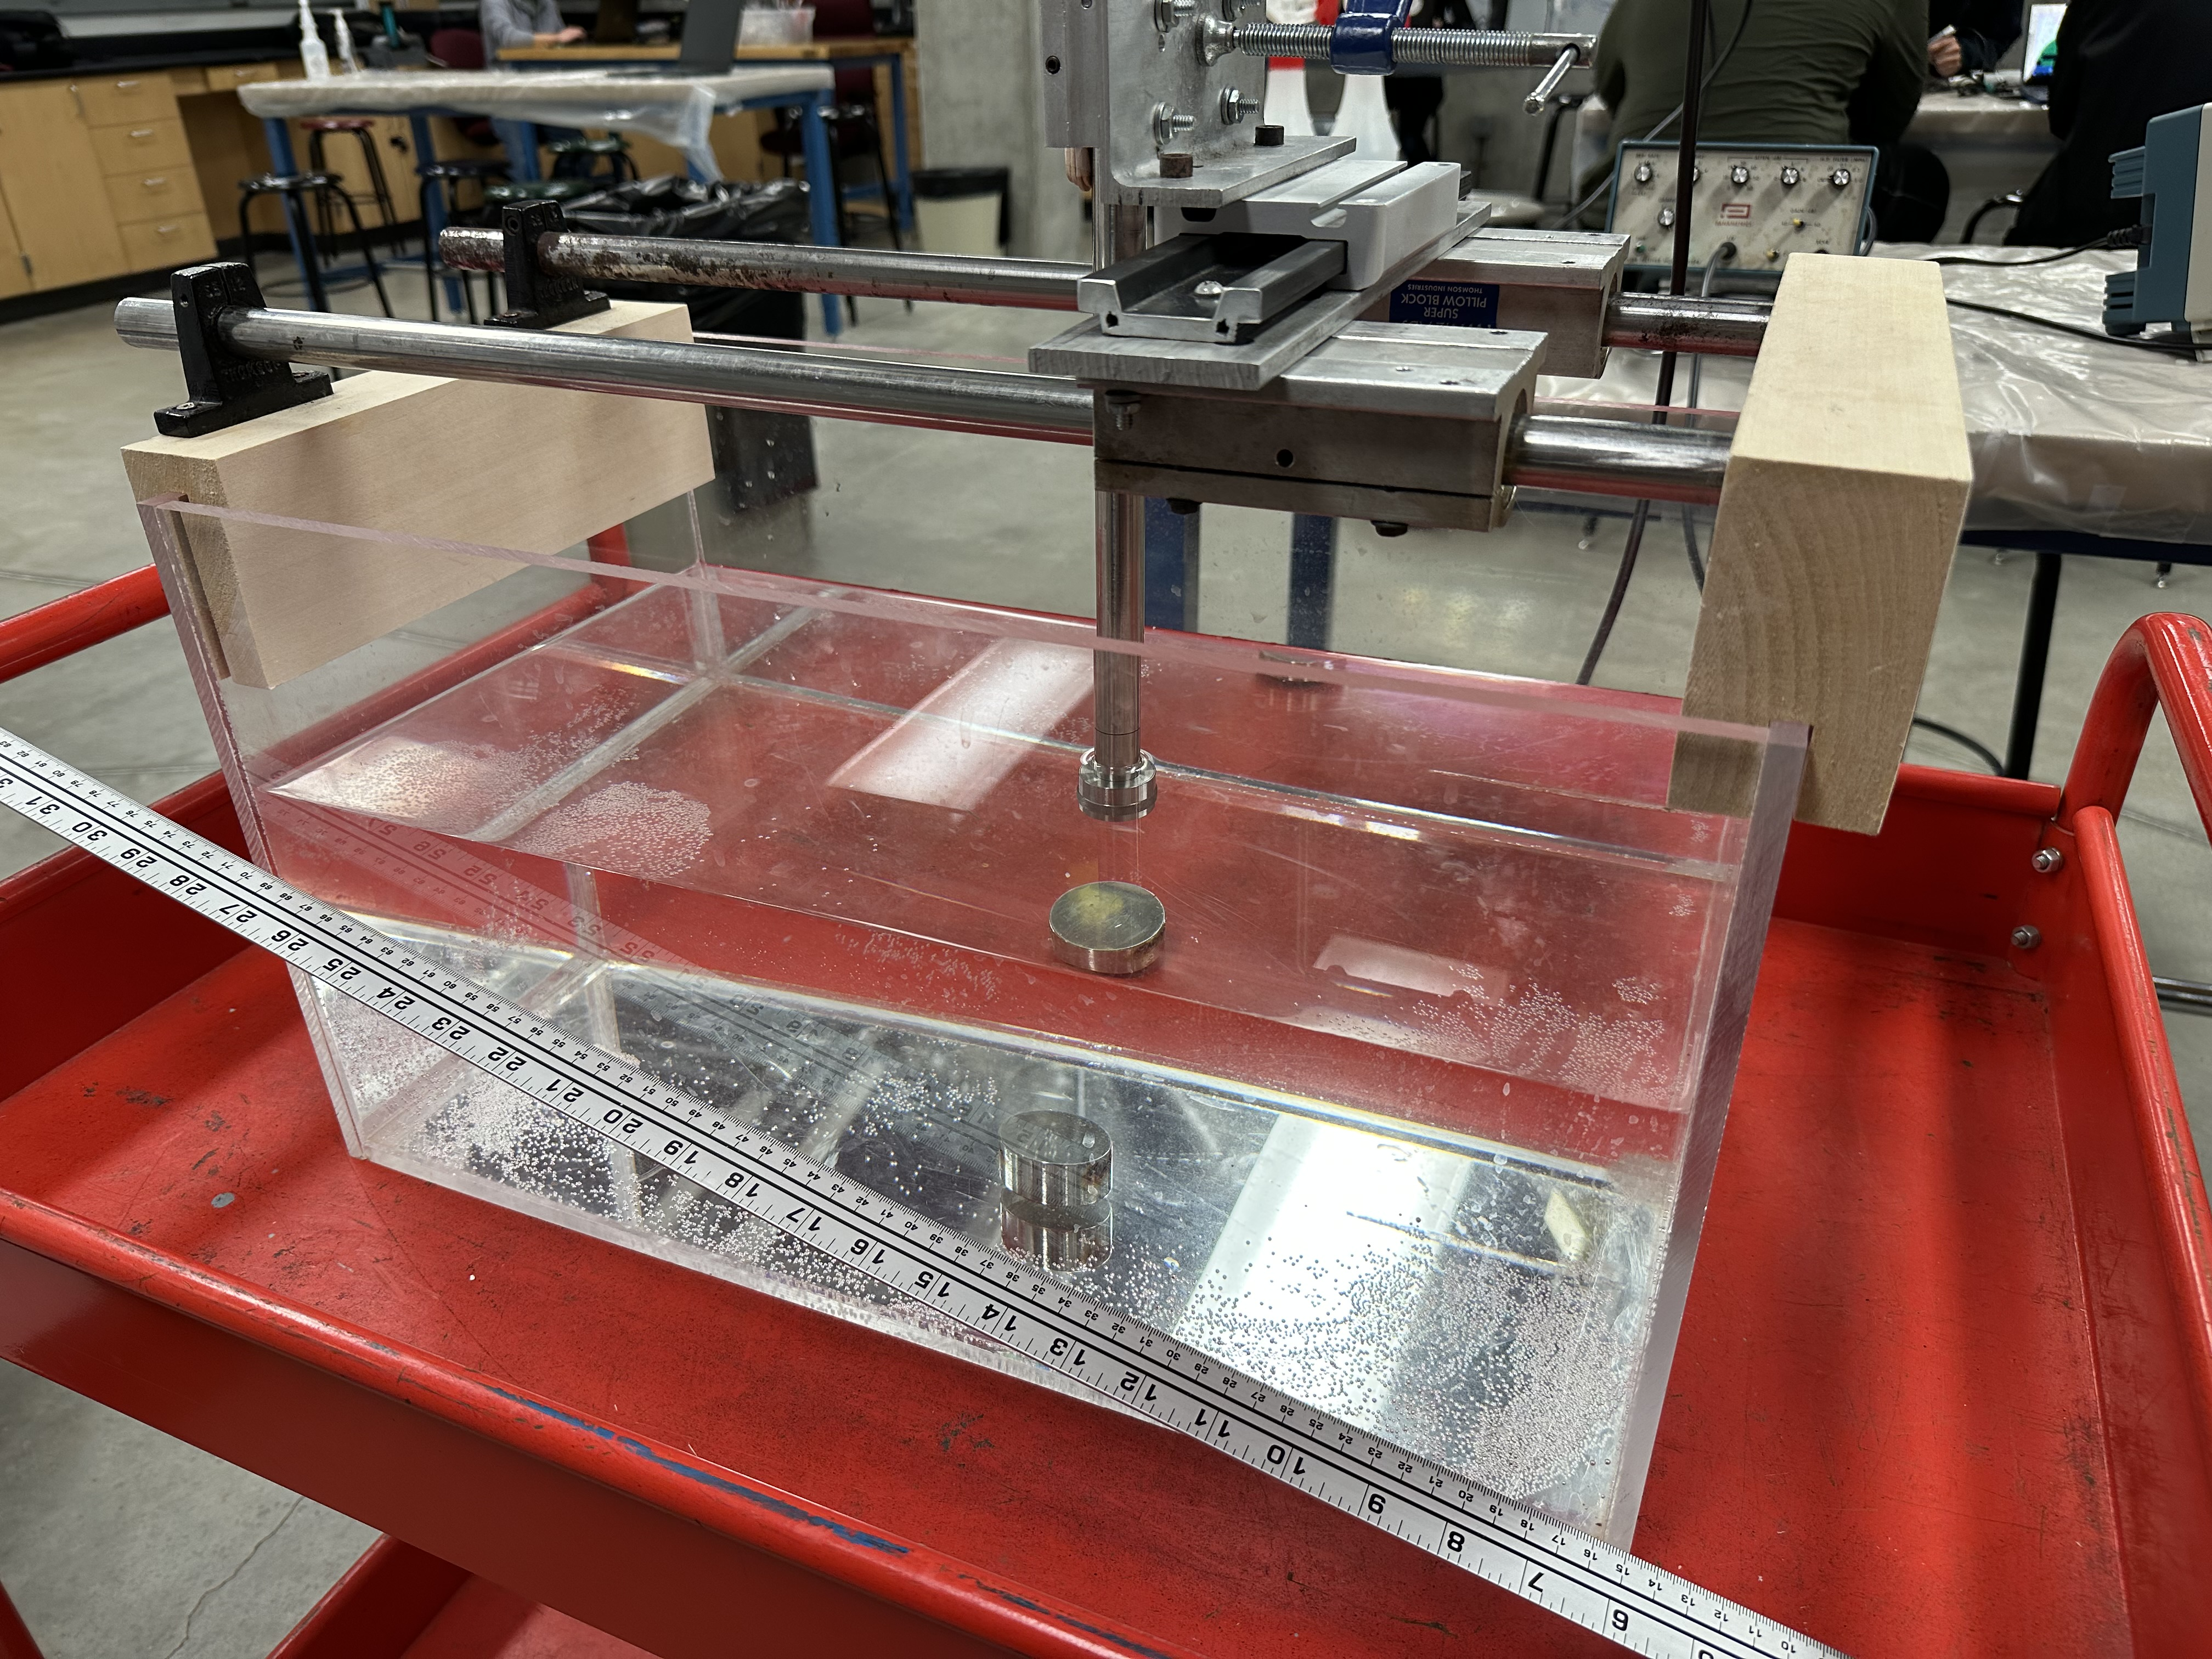
\includegraphics[width=4in]{images/ultrasonic_apparatus}
	\caption{The ultrasonic testing apparatus.}
	\label{fig:ultrasonic_apparatus}
\end{figure}

The transducer is connected to a pulser/receiver which is then connected to an oscilloscope that visualizes the pulses. Figure \ref{fig:oscilloscope} shows the main display of the oscilloscope.

\begin{figure}[htbp]
	\centering
	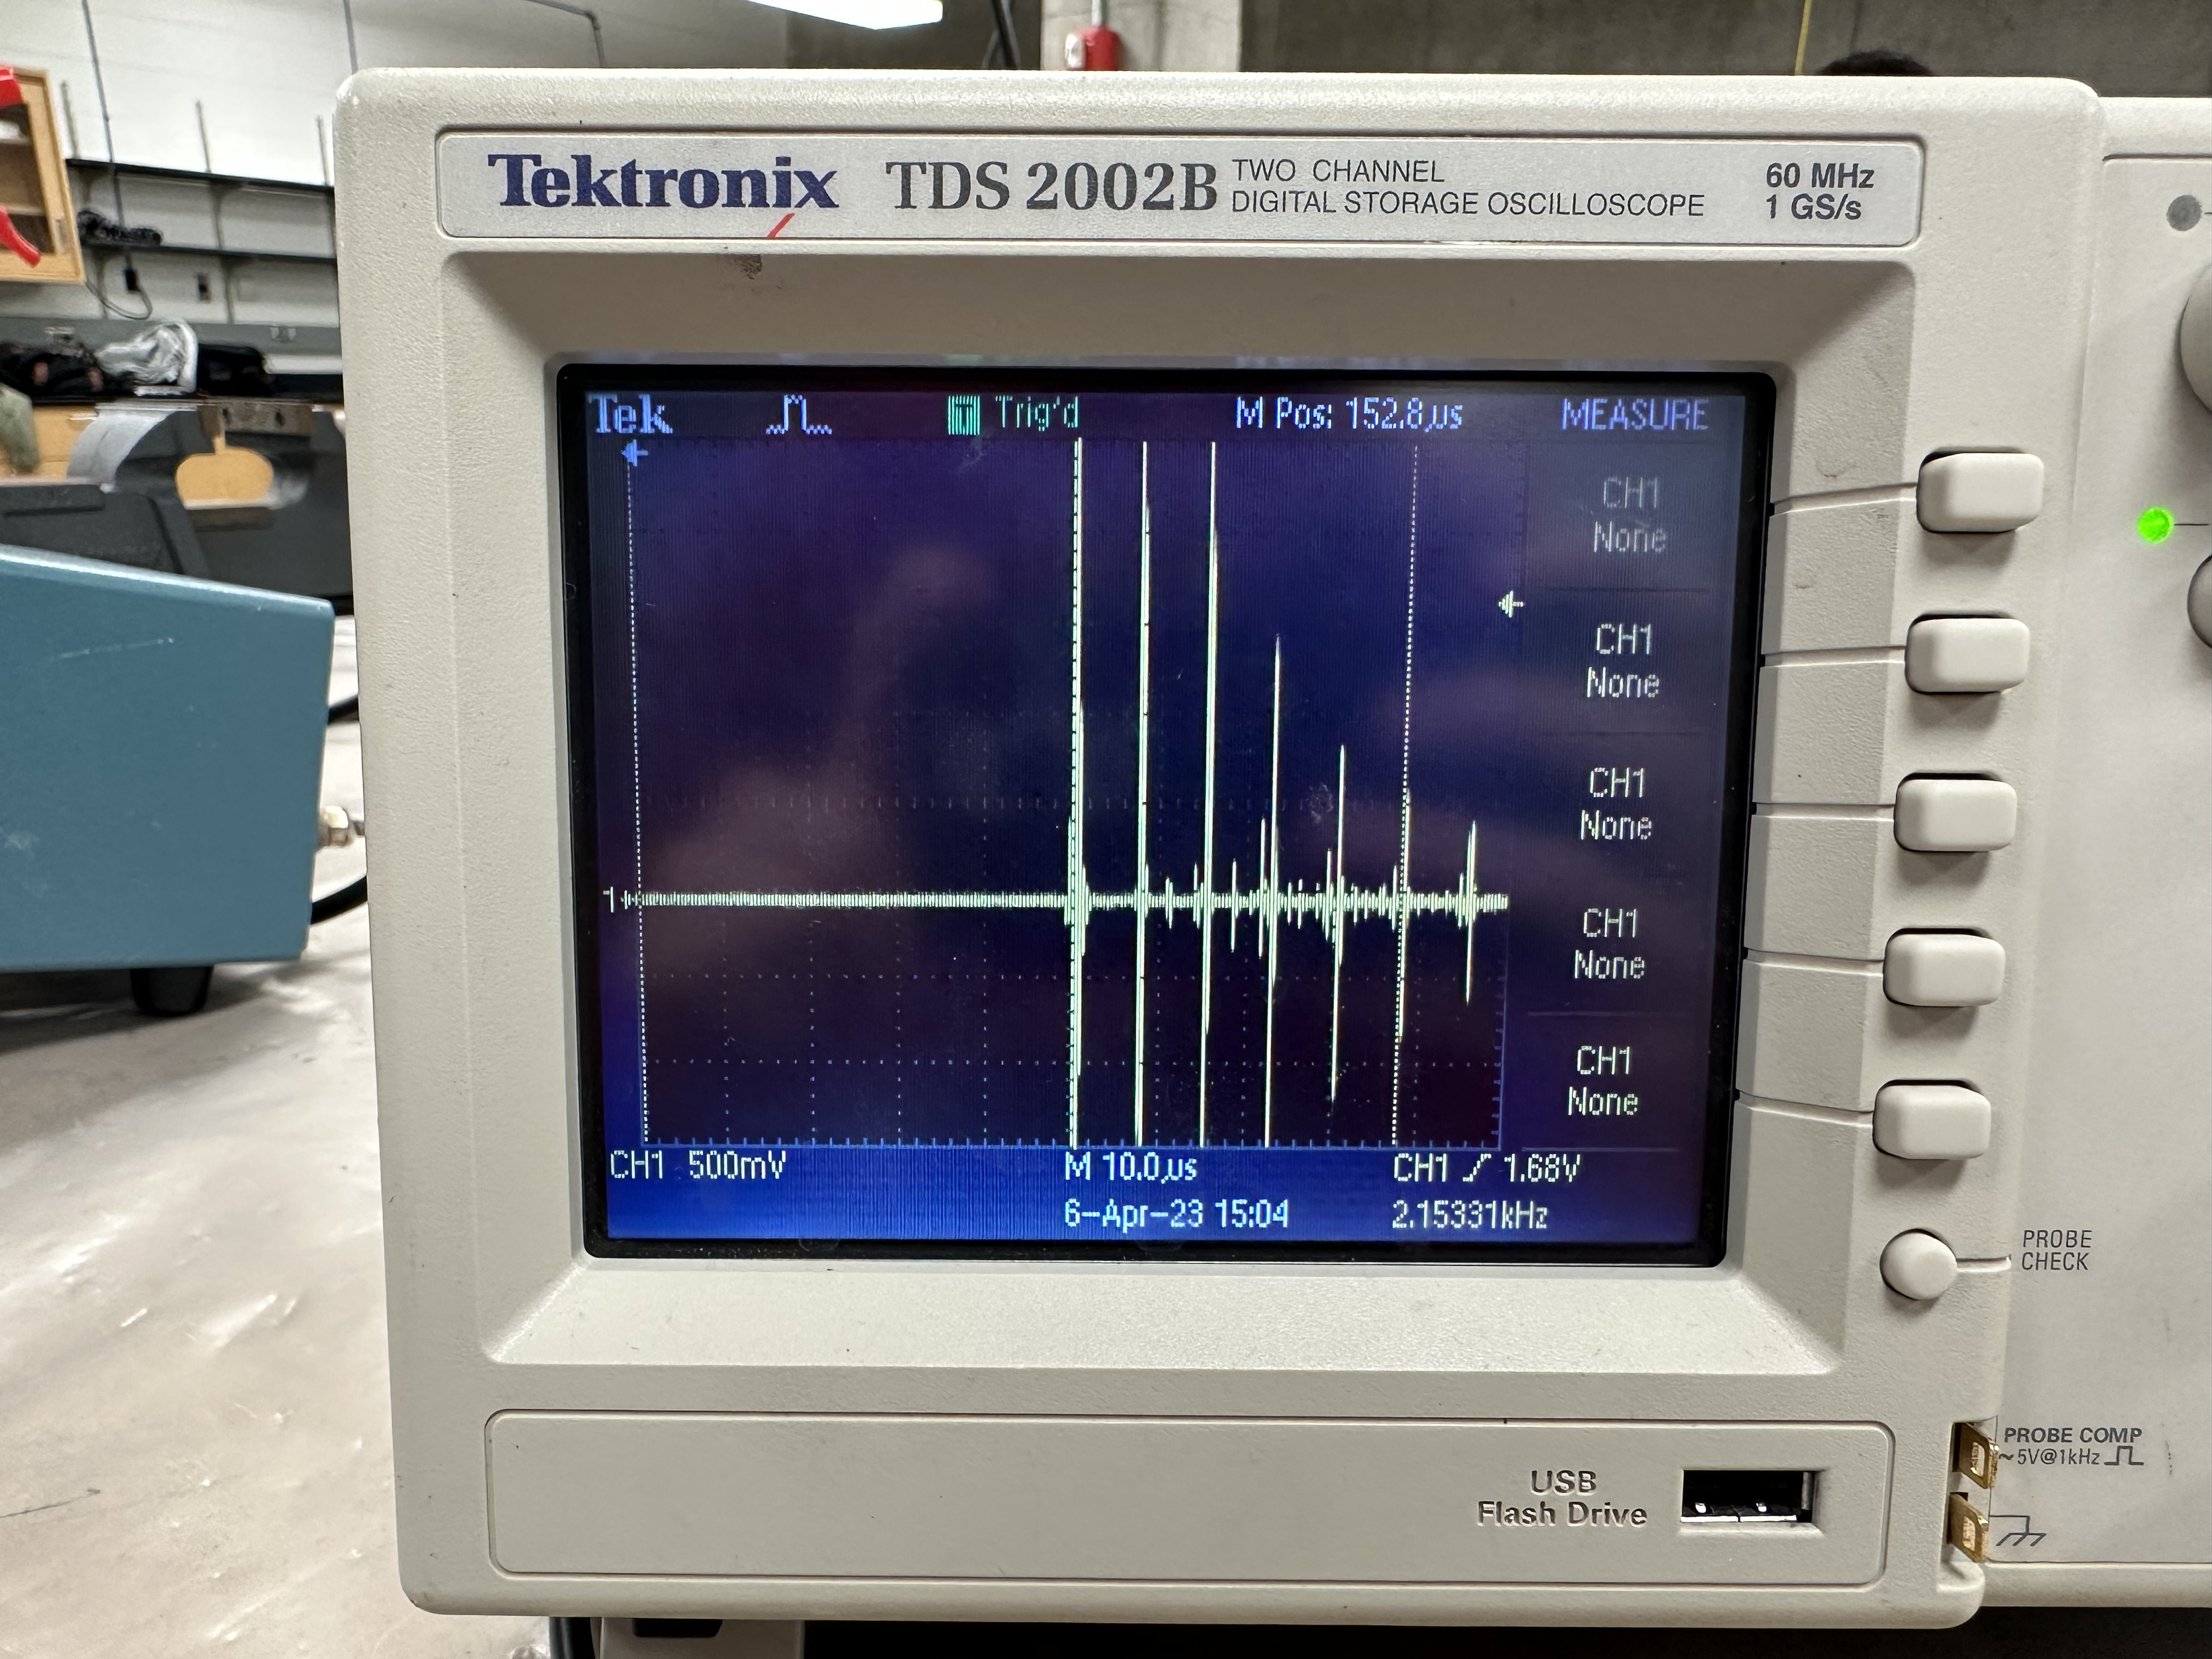
\includegraphics[width=4in]{images/oscilloscope}
	\caption{The display on the oscilloscope.}
	\label{fig:oscilloscope}
\end{figure}

\textbf{Simulated Ultrasonic Testing}

The UT\_SN\_Sim software was used for the ultrasonic simulation testing. The initial configuration of the software is shown in Figures \ref{fig:sim_1} through \ref{fig:sim_8}.

\begin{figure}[htbp]
	\centering
	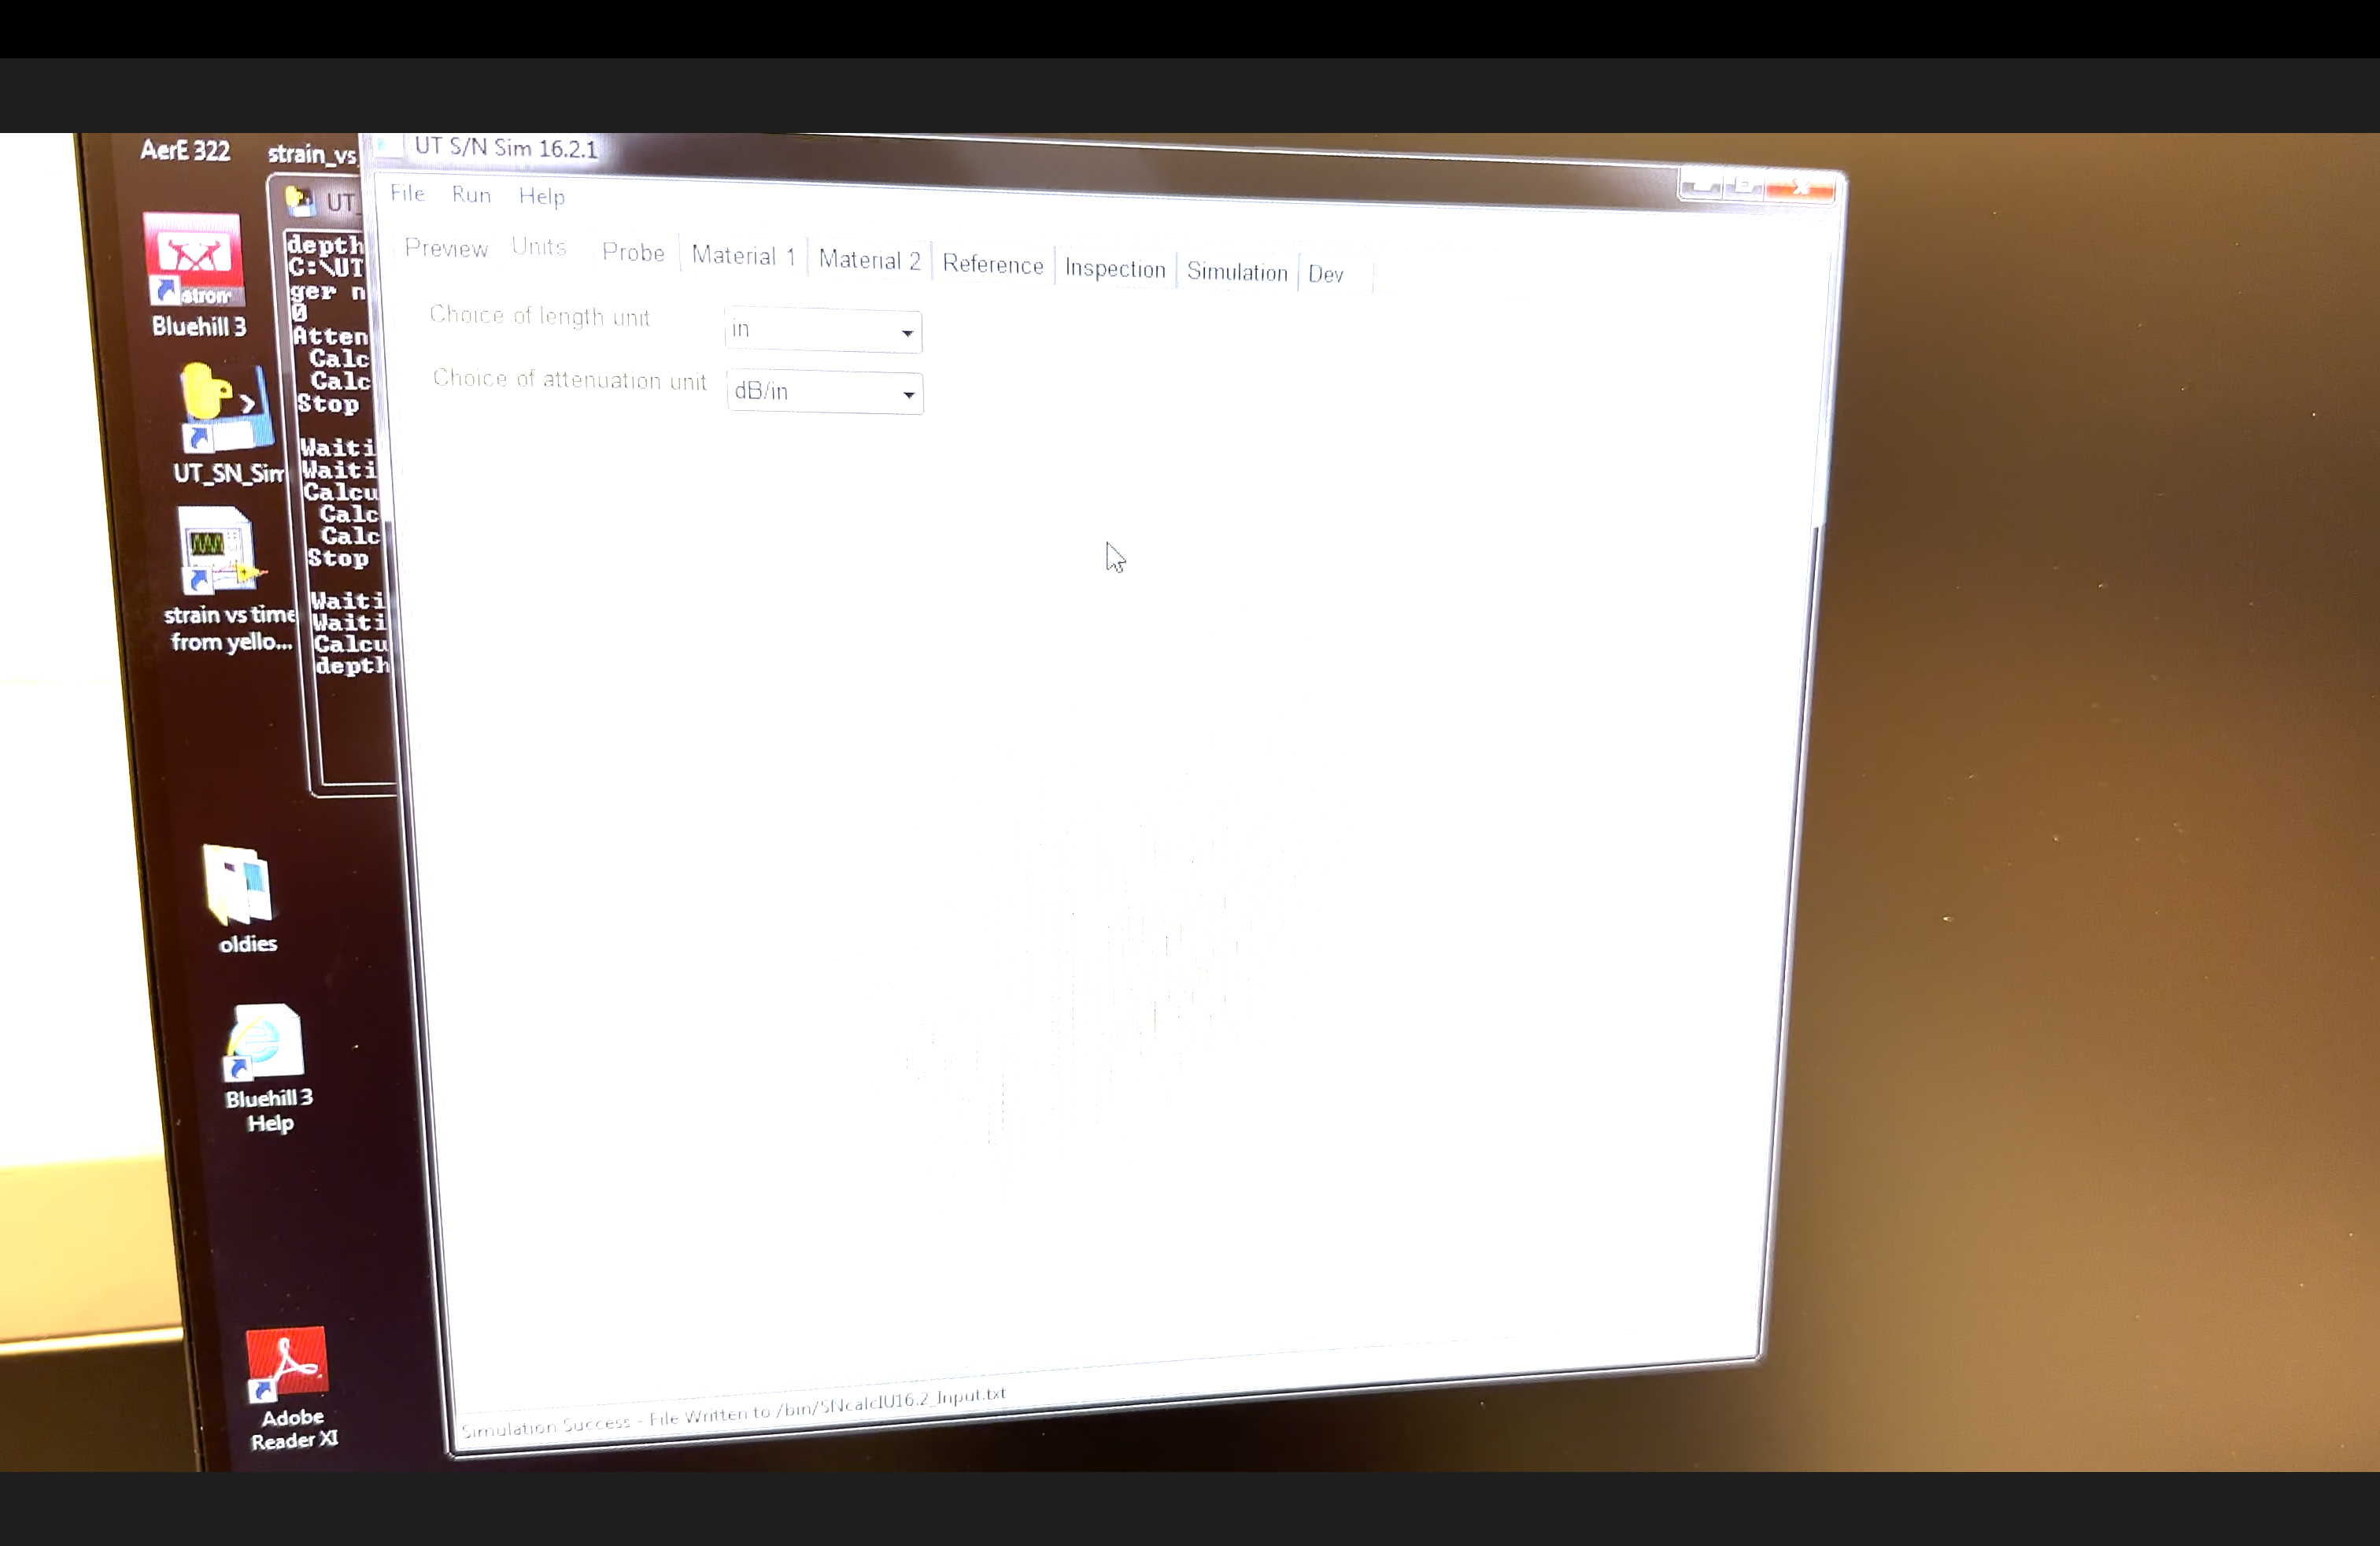
\includegraphics[width=4in]{images/sim_1}
	\caption{The units configuration page of the ultrasonic simulation software.}
	\label{fig:sim_1}
\end{figure}

\begin{figure}[htbp]
	\centering
	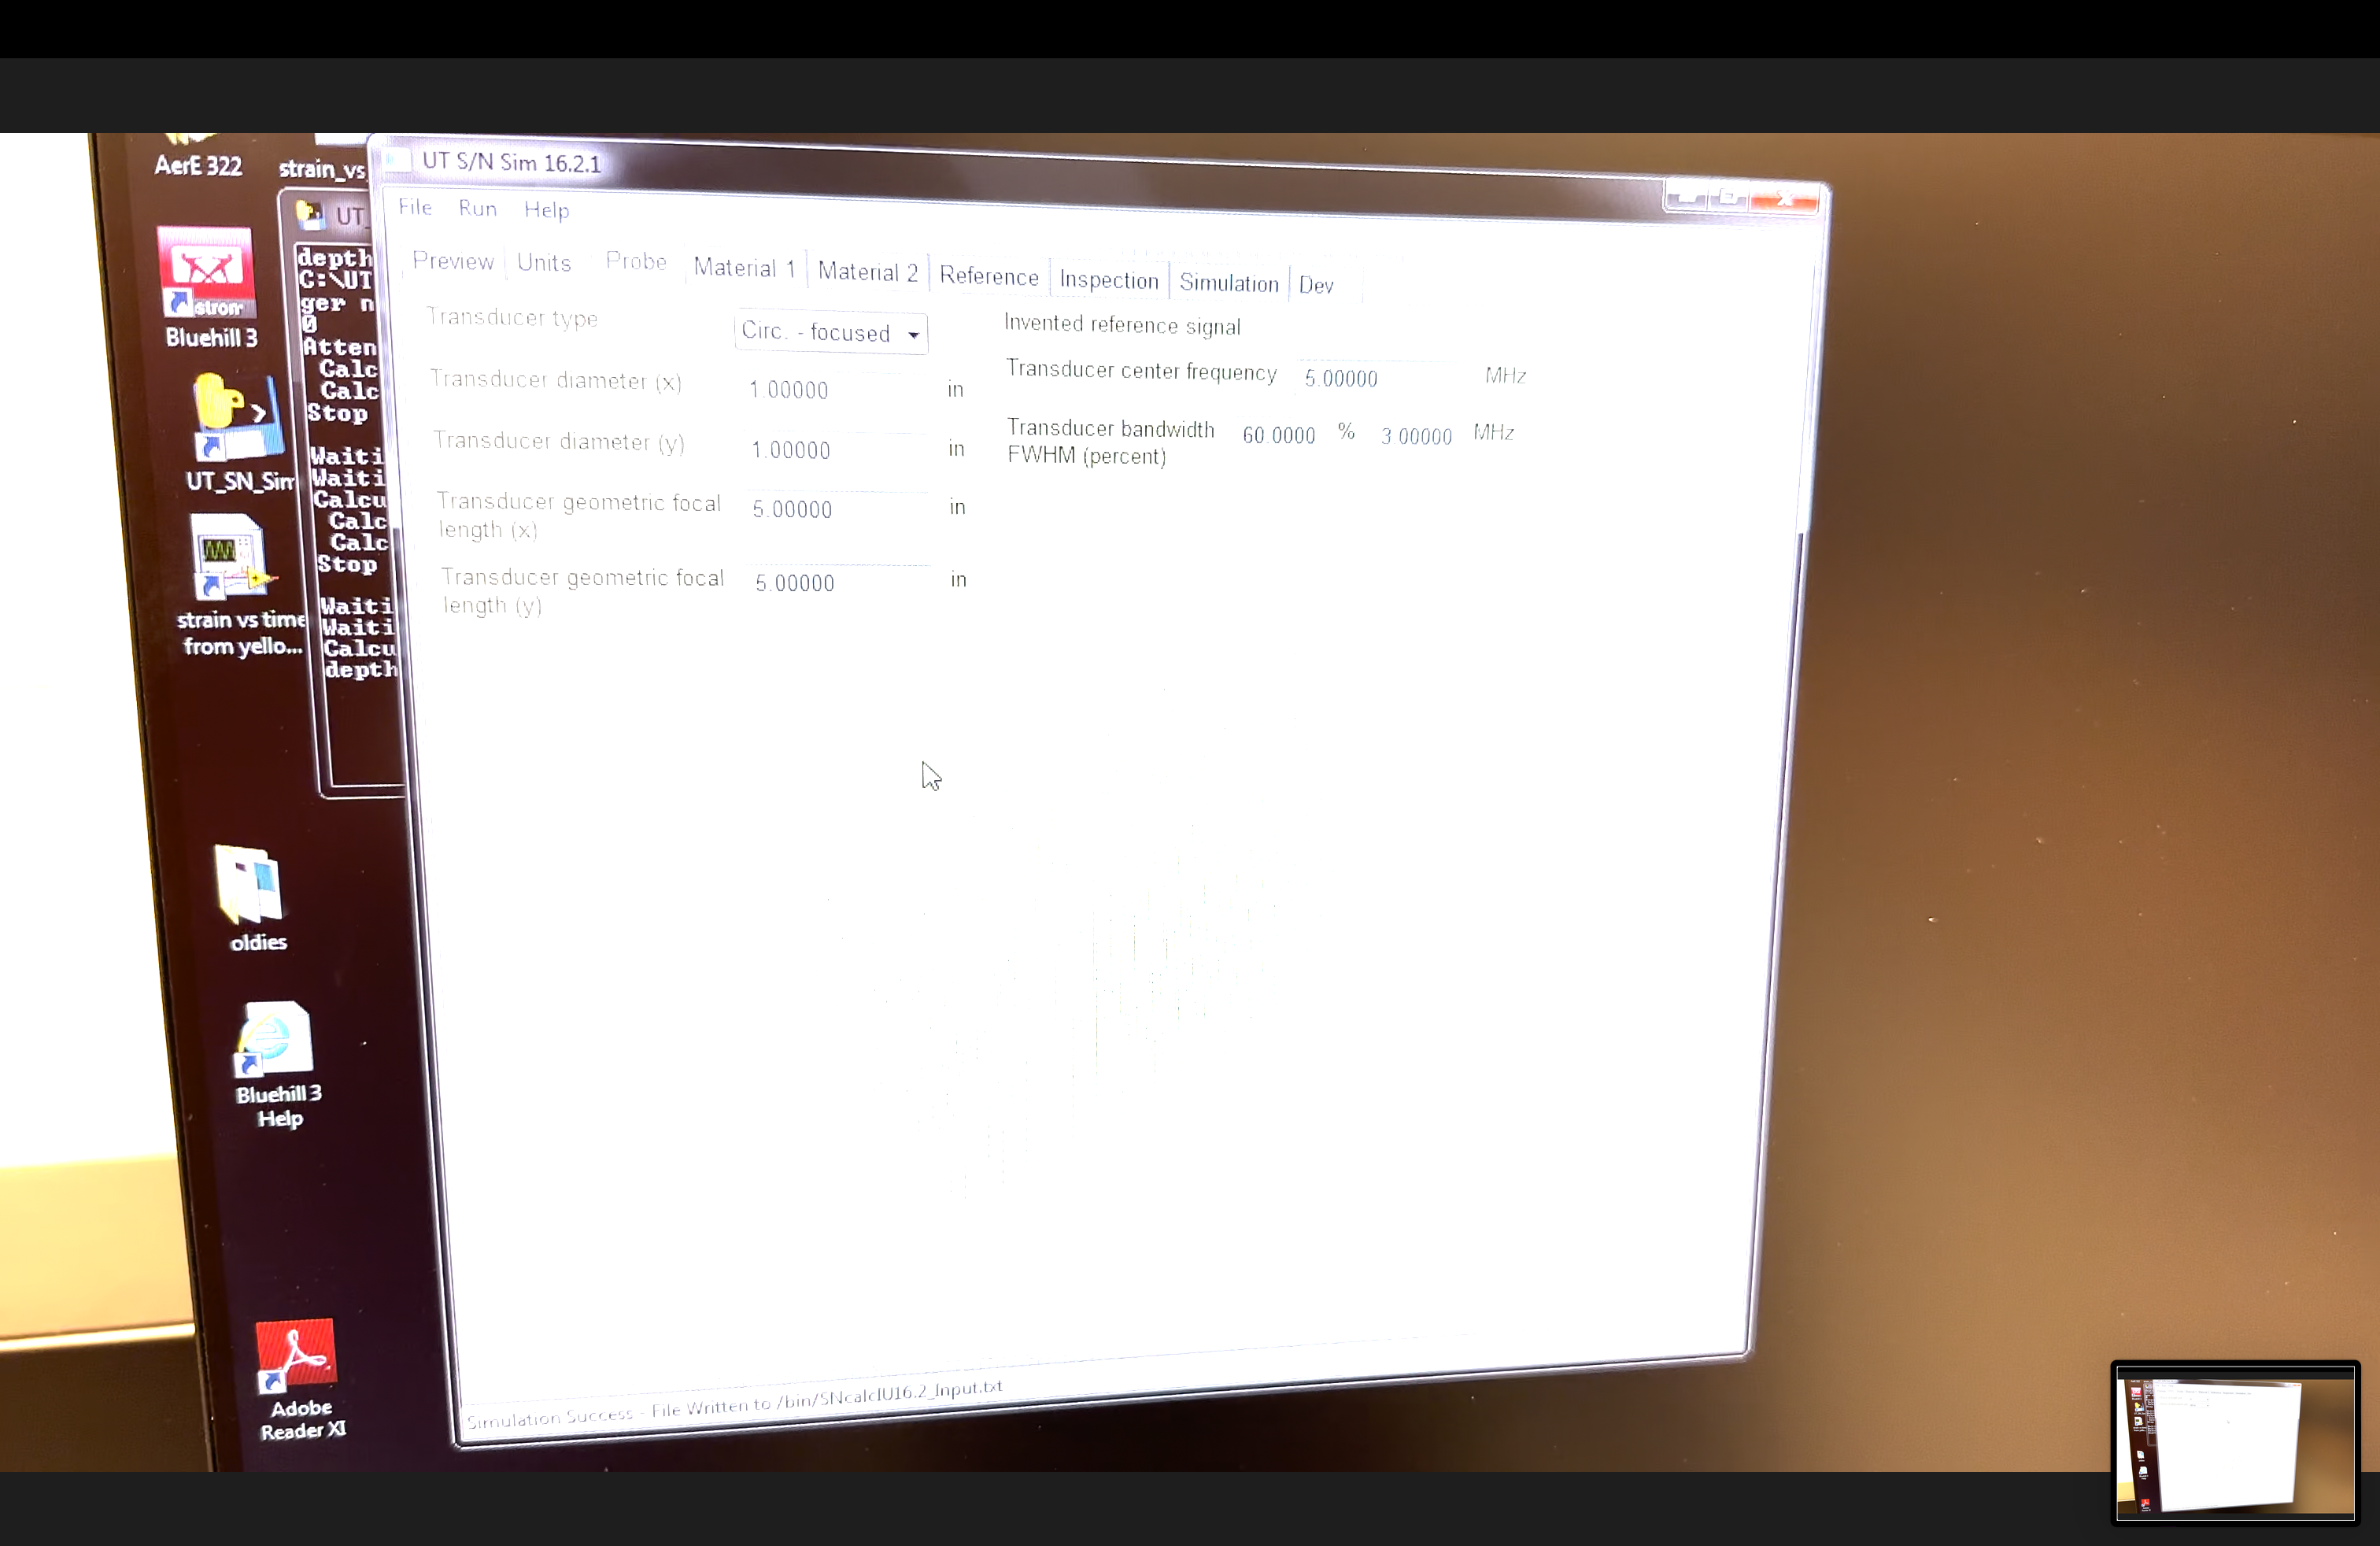
\includegraphics[width=4in]{images/sim_2}
	\caption{The probe configuration page of the ultrasonic simulation software.}
	\label{fig:sim_2}
\end{figure}

\begin{figure}[htbp]
	\centering
	\includegraphics[width=4in]{images/sim_3}
	\caption{The material \num{1} configuration page of the ultrasonic simulation software.}
	\label{fig:sim_3}
\end{figure}

\begin{figure}[htbp]
	\centering
	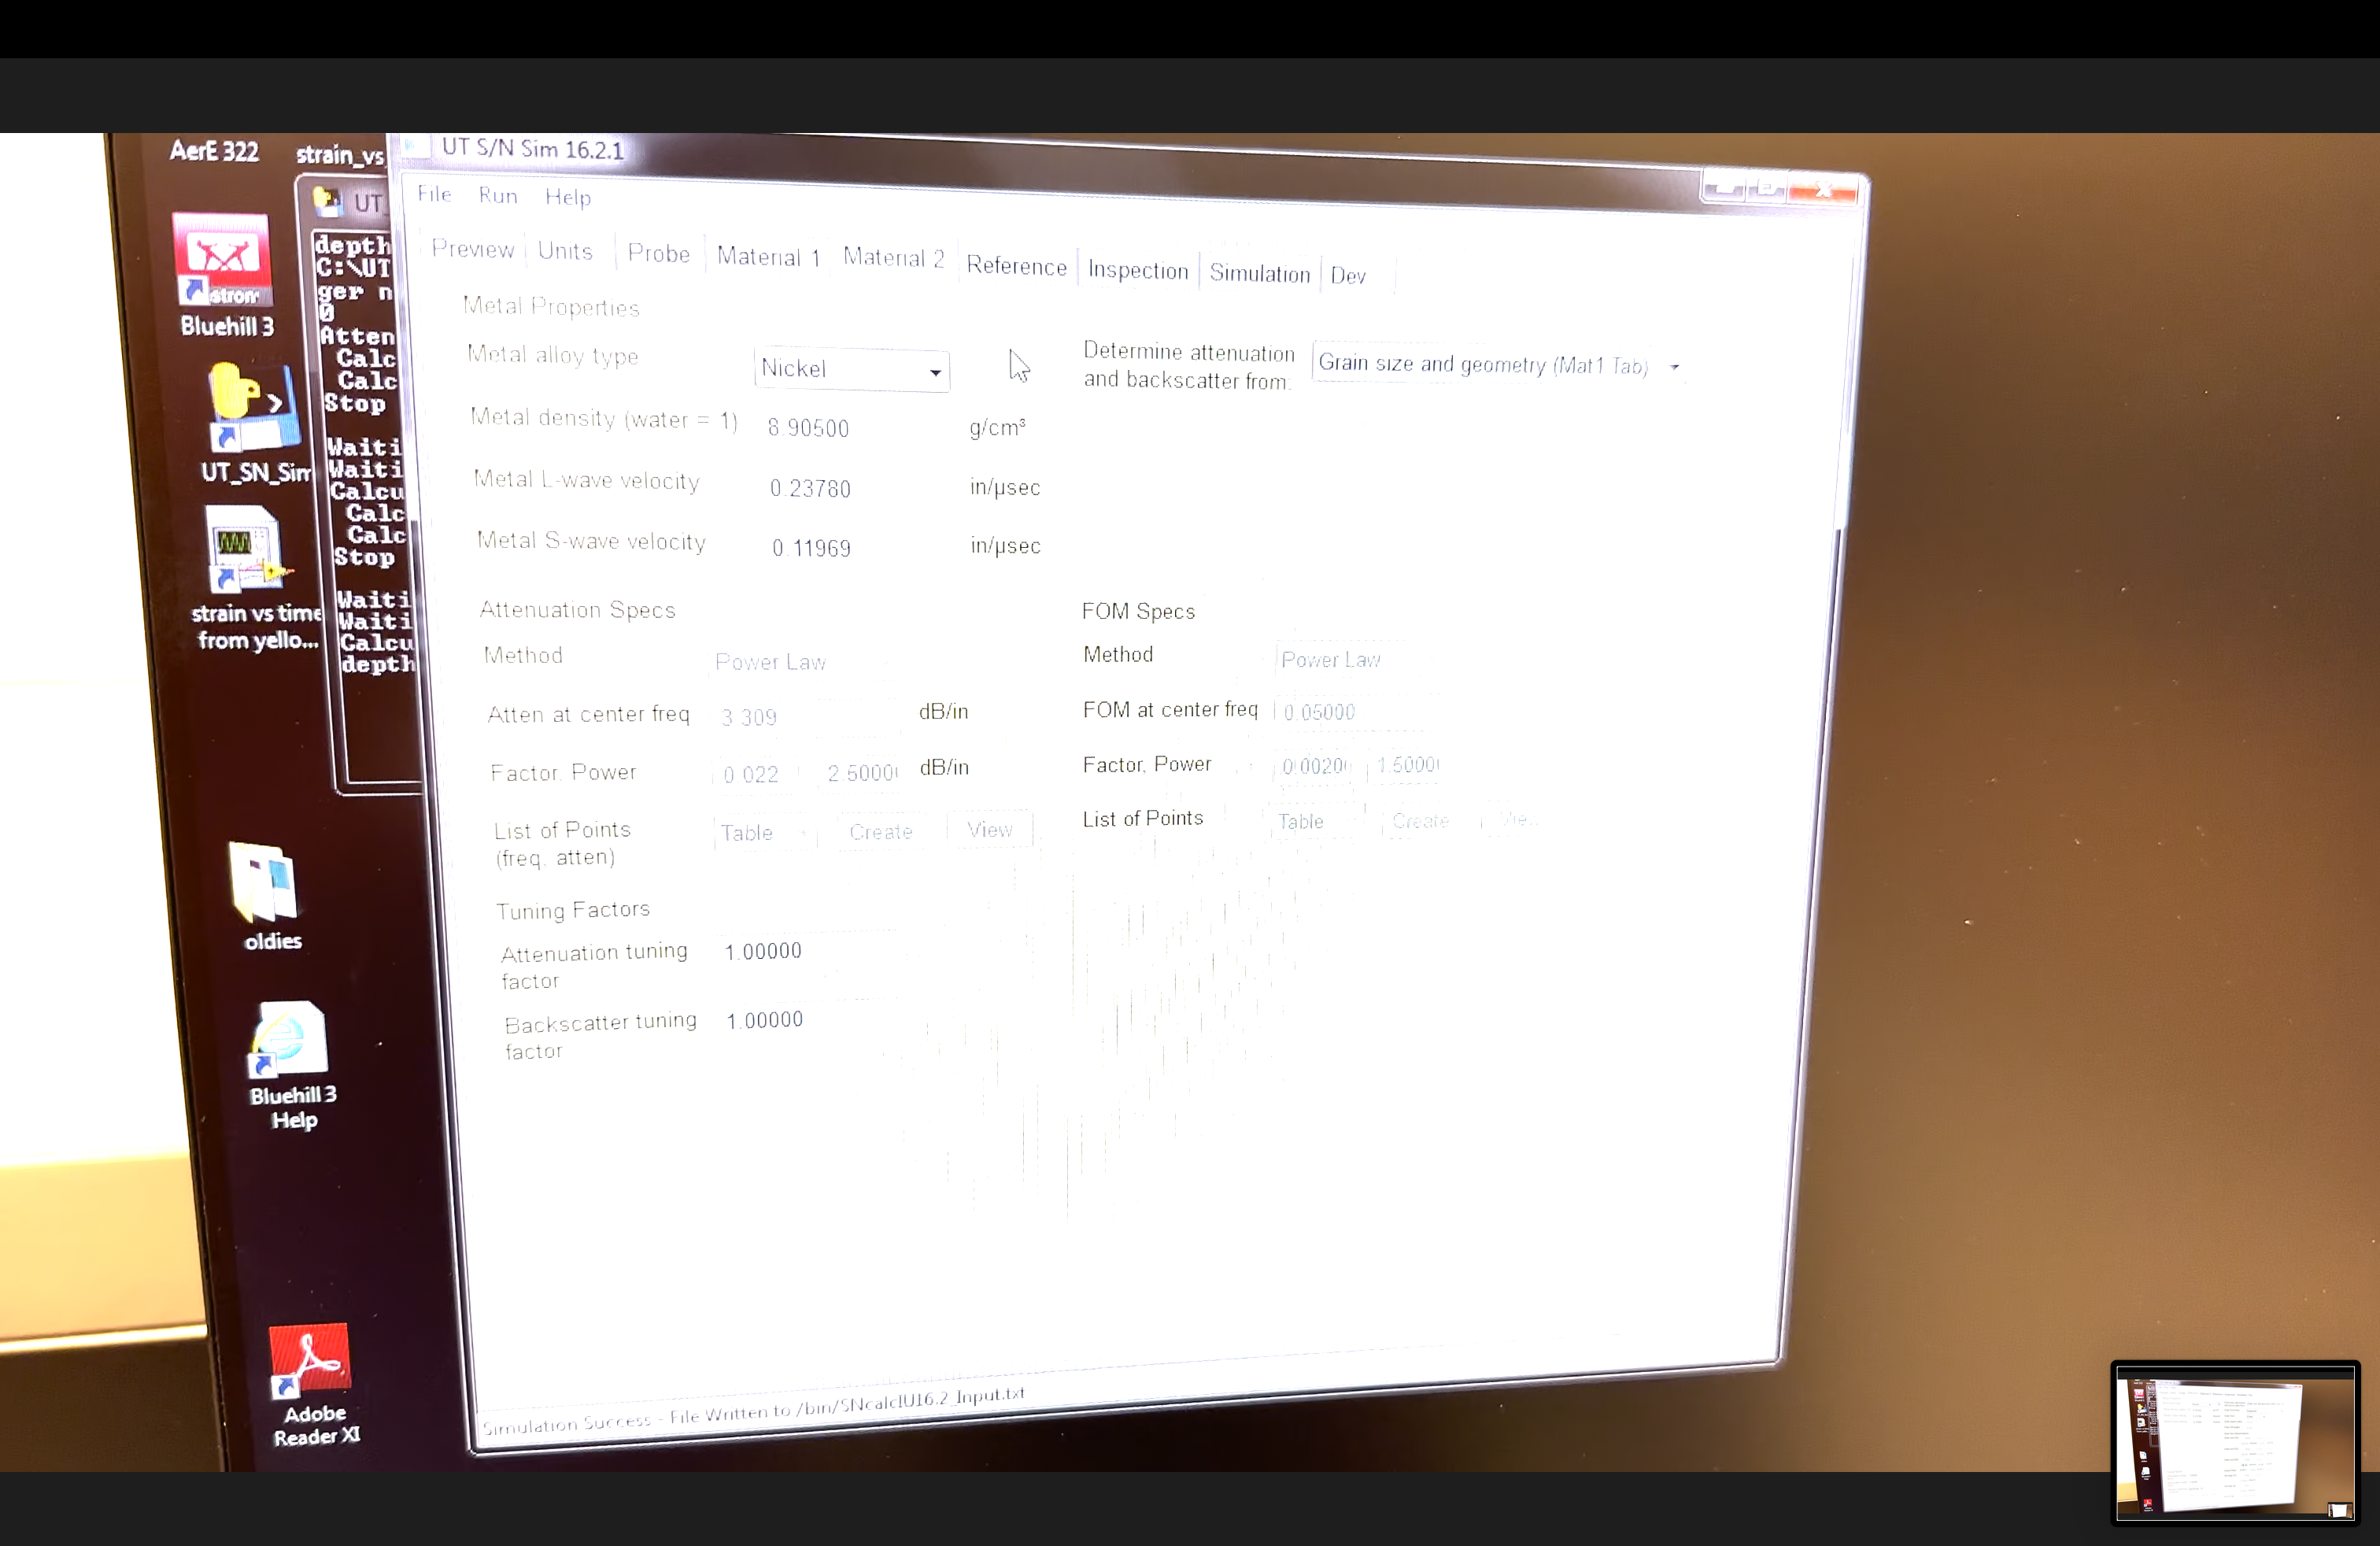
\includegraphics[width=4in]{images/sim_4}
	\caption{The material \num{2} configuration page of the ultrasonic simulation software.}
	\label{fig:sim_4}
\end{figure}

\begin{figure}[htbp]
	\centering
	\includegraphics[width=4in]{images/sim_5}
	\caption{The reference configuration page of the ultrasonic simulation software.}
	\label{fig:sim_5}
\end{figure}

\begin{figure}[htbp]
	\centering
	\includegraphics[width=4in]{images/sim_6}
	\caption{The inspection configuration page of the ultrasonic simulation software.}
	\label{fig:sim_6}
\end{figure}

\begin{figure}[htbp]
	\centering
	\includegraphics[width=4in]{images/sim_7}
	\caption{The simulation configuration page of the ultrasonic simulation software.}
	\label{fig:sim_7}
\end{figure}

\begin{figure}[htbp]
	\centering
	\includegraphics[width=4in]{images/sim_8}
	\caption{The dev configuration page of the ultrasonic simulation software.}
	\label{fig:sim_8}
\end{figure}

\newpage

\textbf{Eddy Current Testing}

The eddy current testing apparatus consists of two aluminum samples labeled BKI and BKII and a variety of different metal pucks of different material. An EddyCation interface box is attached to a computer running the EddyCation software as well as an absolute probe that is used to perform the eddy current testing. The BKI sample will be tested right-side up and upside-down, but the BKII sample will be tested exclusively with the notches facing the table. The BKI and BKII samples are shown in Figure \ref{fig:eddy_current_apparatus} as well as the metal samples in the background.

\begin{figure}[htbp]
	\centering
	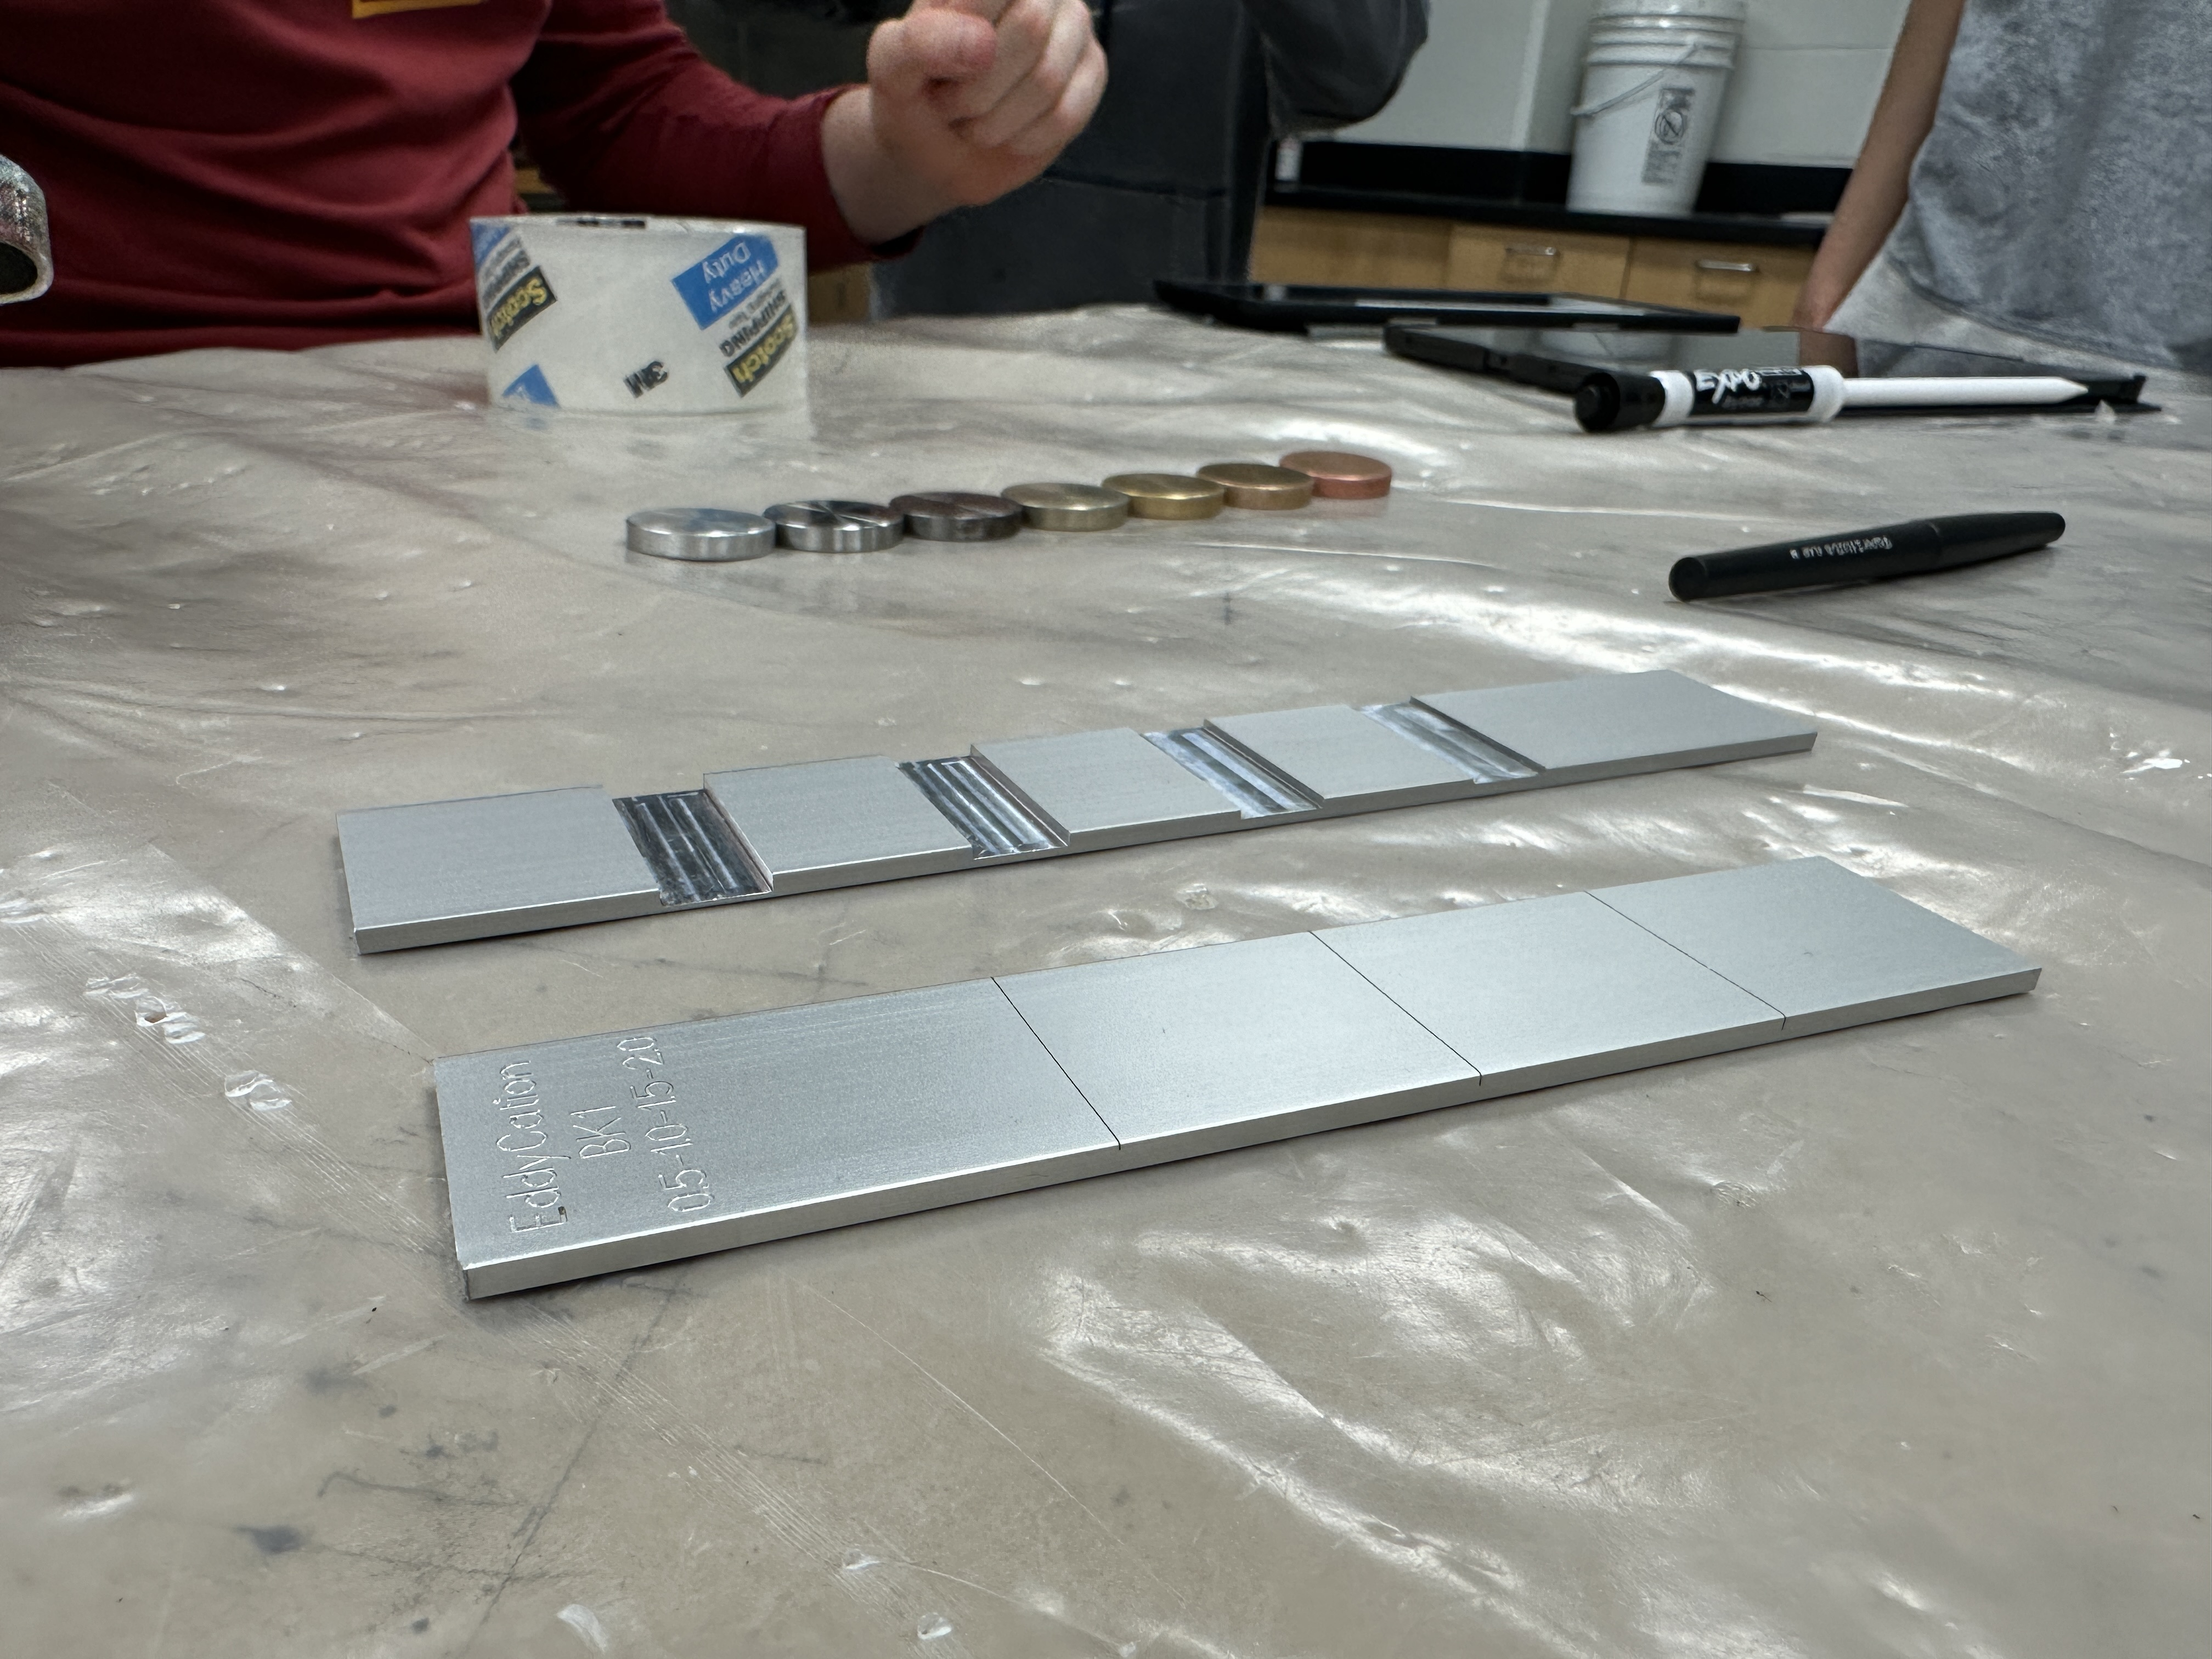
\includegraphics[width=4in]{images/eddy_current_apparatus}
	\caption{The BKI sample (front), BKII sample (middle), and metal samples (back) for the eddy current testing lab.}
	\label{fig:eddy_current_apparatus}
\end{figure}

\textbf{Tap Testing}

The tap testing will take place on a \qtyproduct{10.5x12}{in} honey comb defect area plate. The hand tapper is connected to an electronics box which is further connected to a computer running the CATT software. The clear grid is placed over the material to help the tester position their tap placements. The overall tap testing configuration is shown in Figure \ref{fig:tap_testing_apparatus} and the software configuration is shown in Figure \ref{fig:tap_testing_software}.

\begin{figure}[htbp]
	\centering
	\includegraphics[width=4in]{images/tap_testing_apparatus}
	\caption{The tap testing lab apparatus.}
	\label{fig:tap_testing_apparatus}
\end{figure}

\begin{figure}[htbp]
	\centering
	\includegraphics[width=4in]{images/tap_testing_software}
	\caption{The software configuration for the tap testing lab.}
	\label{fig:tap_testing_software}
\end{figure}

\section{Procedures} \label{procedures}
\textbf{Ultrasonic Testing}

First start by calculating how far the transducer face needs to be from the defect on the bottom face of the sample and adjust the height of the transducer accordingly. Twist the horizontal position knob to move across the time scale and see the waves. Adjust the vertical and horizontal position to clearly see the waves. From here, move the transducer along both the “x” and “y” axies of the track over the sample. There will be a clear change in waves, for our group the second wave being displayed on the oscilloscope. Observe how the wave changes to determine the edge of the defect. This will be located at the point of maximum volt amplitude. Measure the position of the transducer against a reference point and move the transducer until the other edge is found. Measure the position of the transducer once again. Take the difference between the two measurements and this give you the diameter of the defect in one direction. Repeat the same process but in the other direction to find “both” diameters.

\textbf{Simulated Ultrasonic Testing}

Turn on the simulator by clicking play as the first process. After some seconds, the home screen will be appeared. As the basic setting, we will modify some parameters. In simulation Tab, set Defect type to FBH and re-enter defect size to 1/64 inches. In material 1 tab, set the metal alloy type to nickel and enter grain size to 100 microns. In Inspection tab, set wave mode in metal to longitude mode. We can change the following parameters to get a suitable result: transducer type, transducer diameter, focal length, Cener frequency, water path, and Bandwidth. After setting parameters above and getting ready to execute test, click run simulation button, and we can see the result of test. At first, defect signal amplitude and grain noise amplitude will be shown on the top of the result view, using different y axis scale. On the middle, graph of signal noise ratio versus depth will be shown. Additionally, we can see the graphs of 2 A scan with different approach by clicking the point on the line shown on the top graph. We will have to repeat those process until we find the parameter dominating the result of plots.

\textbf{Eddy Current Testing}

Set up the testing software, then adjust the frequency below 10 KHz to compensate for the cracks being on the top of the BKI sample. Also adjust the phase angle so that it is tracing the left side of the resistance axis. Then adjust the gain to below 45 dB and the low pass bandwidth frequency to 15. Once all settings are correct, perform a lift off calibration to fine tune the phase angle and center the trace. Then slide the probe across the sample, changing the trace color after going over each crack to have each crack distinguishable.

For testing the backside of the BKI sample, the frequency needs to be lowered slightly to have the probe be more sensitive to “deeper” cracks. The process is exactly the same as testing the front side of the sample for testing the back side. Adjust the gain and phase angle accordingly, then perform a lift off calibration. Then slide the probe across the sample, changing the color of the trace after each crack is passed. For the backside of the sample the gain may need to be raised slightly for the trace to be clearer.

The BKII sample is only being tested on the back side. Follow the process described above, adjusting phase angle, frequency, and gain to get clear data. Then slide the probe along the sample and change the color of the trace to distinguish between each gap.

To sort the metal samples, make the necessary adjustments to phase angle, frequency, and gain. Perform a lift off calibration on the first sample and center the trace. From here you can hop from sample to sample using the probe. Observe how each sample leaves a different trace.

\textbf{Tap Testing}

Firstly, set up the tap test software, and try a few gentle taps on the surface, holding the tap head on the metal part in the upper position. Take care not to tap strongly on the surface, or the tap head will be damaged and affect the test result. After checking, tape a plastic grid sheet on the specimen, adjusting the end of the cell we will measure. Before starting the test, click the test start button on the software while entering the column and the row number we will tap.

Start to tap from the top and leftmost cell and continue by tapping a cell along a row. After tapping all cells in a row, move to the cell located leftmost in the next row, and continue to do it until the last row. When the test is finished, check whether tapping errors is shown on the screen, and fix errors by re-tapping the same cell. Stop the test by clicking on the button on the software after checking errors, plot the contour of defects, and save the figure as an image on a drive.   

\section{Data} \label{data}
\textbf{Ultrasonic Testing}

For the ultrasonic testing lab, we calculated the optimal water path to be \qty{113.1}{\mm}. Based on this calculation, the time delta from the transducer pulse and the top surface was \qty{152.8}{\micro\second}. Since we know the thickness and wave travel speed through the sample material, we were able to calculate the time delta for the sample to be \qty{7.931}{\micro\second}. Adding these two time deltas together yielded \qty{160.7}{\micro\second}. Just before the pulse at \qty{160.7}{\micro\second} was the location of the defect signal. The script we used to calculate these values is shown in Appendix \ref{apdx:code}.

\textbf{Simulated Ultrasonic Testing}



\textbf{Eddy Current Testing}

For the eddy current testing, we used the configurations shown in Table \ref{tbl:ec} for each test.

\begin{table}[!htbp]
\caption{Software configurations for each of the eddy current tests. Tests one and two used the BKI sample, test three used the BKII sample, and test four used the various metal samples.}
\begin{center}
	\begin{tabular}{cccccc}
		\toprule
		Test&Frequency (\unit{\kilo\hertz})&Gain (\unit{\decibel})&Phase (\unit{\degree})&LP Filter (\unit{\hertz})&HP Filter (\unit{\hertz})\\
		\midrule
		1&\num{5.0}&\num{50.6}&\num{-58.0}&\num{15}&\num{0}\\
		2&\num{3.0}&\num{50.6}&\num{-32.0}&\num{8}&\num{0}\\
		3&\num{3.0}&\num{29.6}&\num{-28.0}&\num{8}&\num{0}\\
		4&\num{3.0}&\num{17.9}&\num{140.5}&\num{8}&\num{0}\\
		\bottomrule
	\end{tabular}
\end{center}
\label{tbl:ec}
\end{table}

The traces for the first test of sample BKI---with the defects open upwards---are shown in Figure \ref{fig:ec_bk1_up}.

\begin{figure}[htbp]
	\centering
	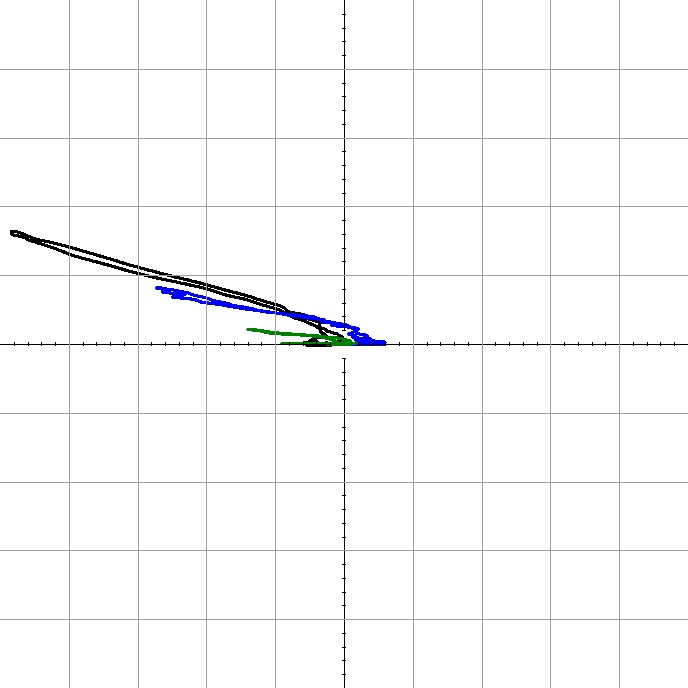
\includegraphics[width=6in]{images/graphs/eddy current testing/S4G2BK1-Upward}
	\caption{The traces recorded from the EddyCation software for the BK1 sample with the defects open upwards.}
	\label{fig:ec_bk1_up}
\end{figure}

The traces for the second test of sample BKI---with the defects open downwards---are shown in Figure \ref{fig:ec_bk1_down}.

\begin{figure}[htbp]
	\centering
	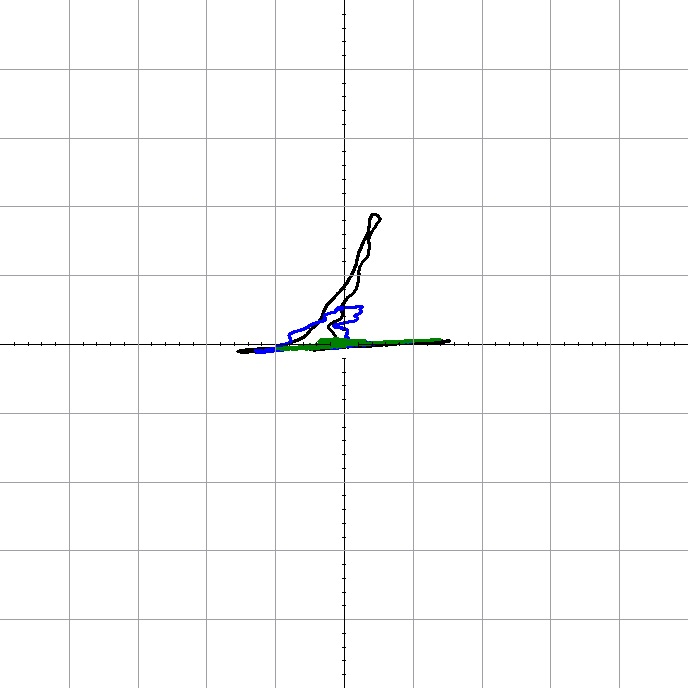
\includegraphics[width=6in]{images/graphs/eddy current testing/S4G2BK1-Downward}
	\caption{The traces recorded from the EddyCation software for the BK1 sample with the defects open downwards.}
	\label{fig:ec_bk1_down}
\end{figure}

The traces for the test of sample BKII are shown in Figure \ref{fig:ec_bk2}.

\begin{figure}[htbp]
	\centering
	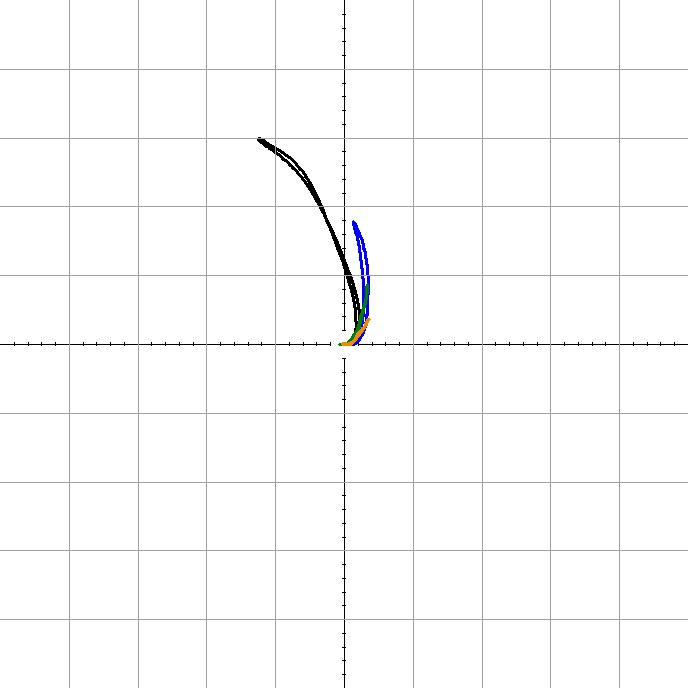
\includegraphics[width=6in]{images/graphs/eddy current testing/S4G2BK2}
	\caption{The traces recorded from the EddyCation software for the BK2 sample.}
	\label{fig:ec_bk2}
\end{figure}

The traces for the metal sample sorting test are shown in Figure \ref{fig:ec_metal_sorting}.

\begin{figure}[htbp]
	\centering
	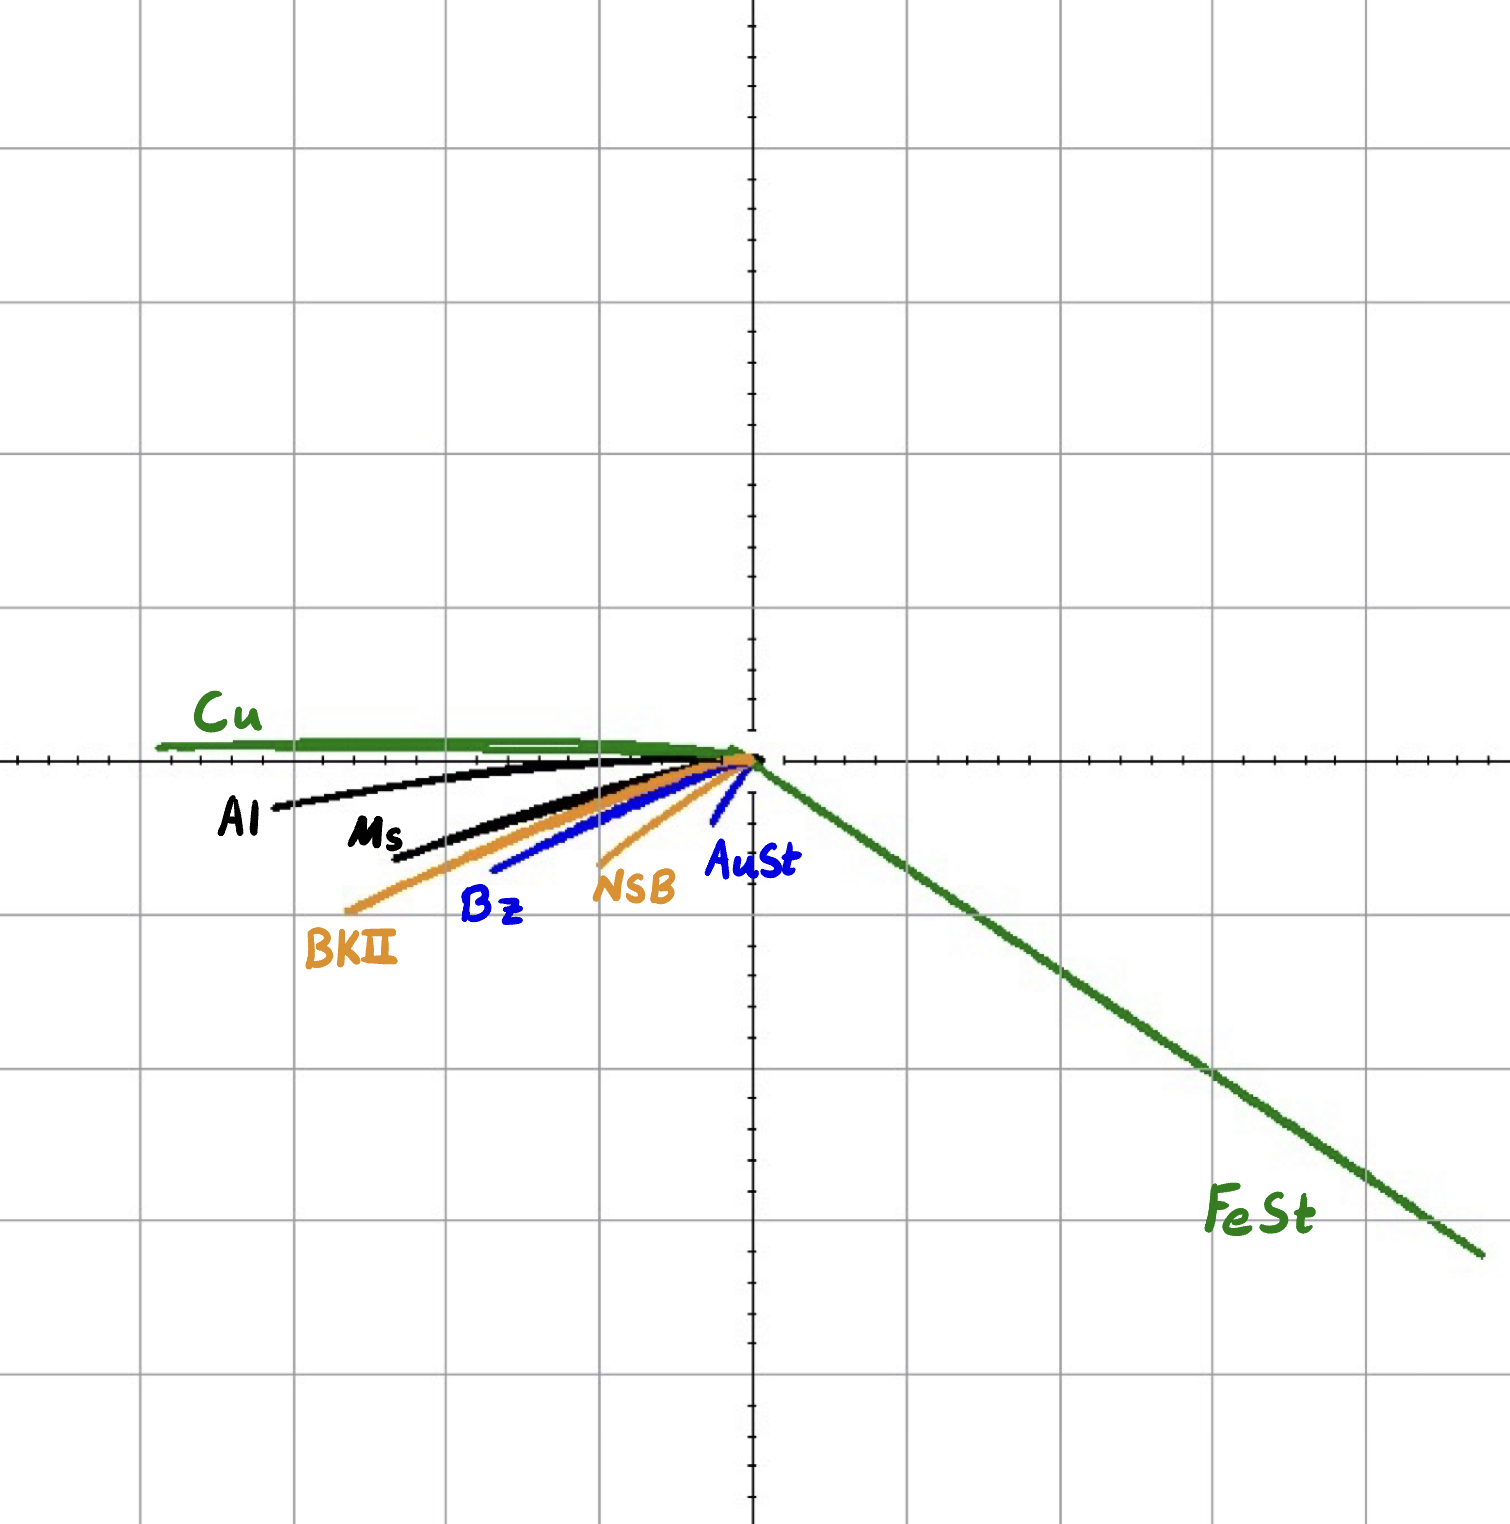
\includegraphics[width=6in]{images/graphs/eddy current testing/S4G2Metal2-labeled}
	\caption{The traces recorded from the EddyCation software for the metal sorting testing. Each trace is labeled according to what metal it is (note: we may have misspelled some of the labels; our notes were not entirely clear).}
	\label{fig:ec_metal_sorting}
\end{figure}

\textbf{Tap Testing}

For the tap testing, we split the sample into two separate tests. The top half of the sample was tested with the first run and the bottom half of the sample was tested with the second run. The orientation of the clear grid and the software configuration for the first tap test run is shown in Figure \ref{fig:tt1_orientation}.

\begin{figure}[htbp]
	\centering
	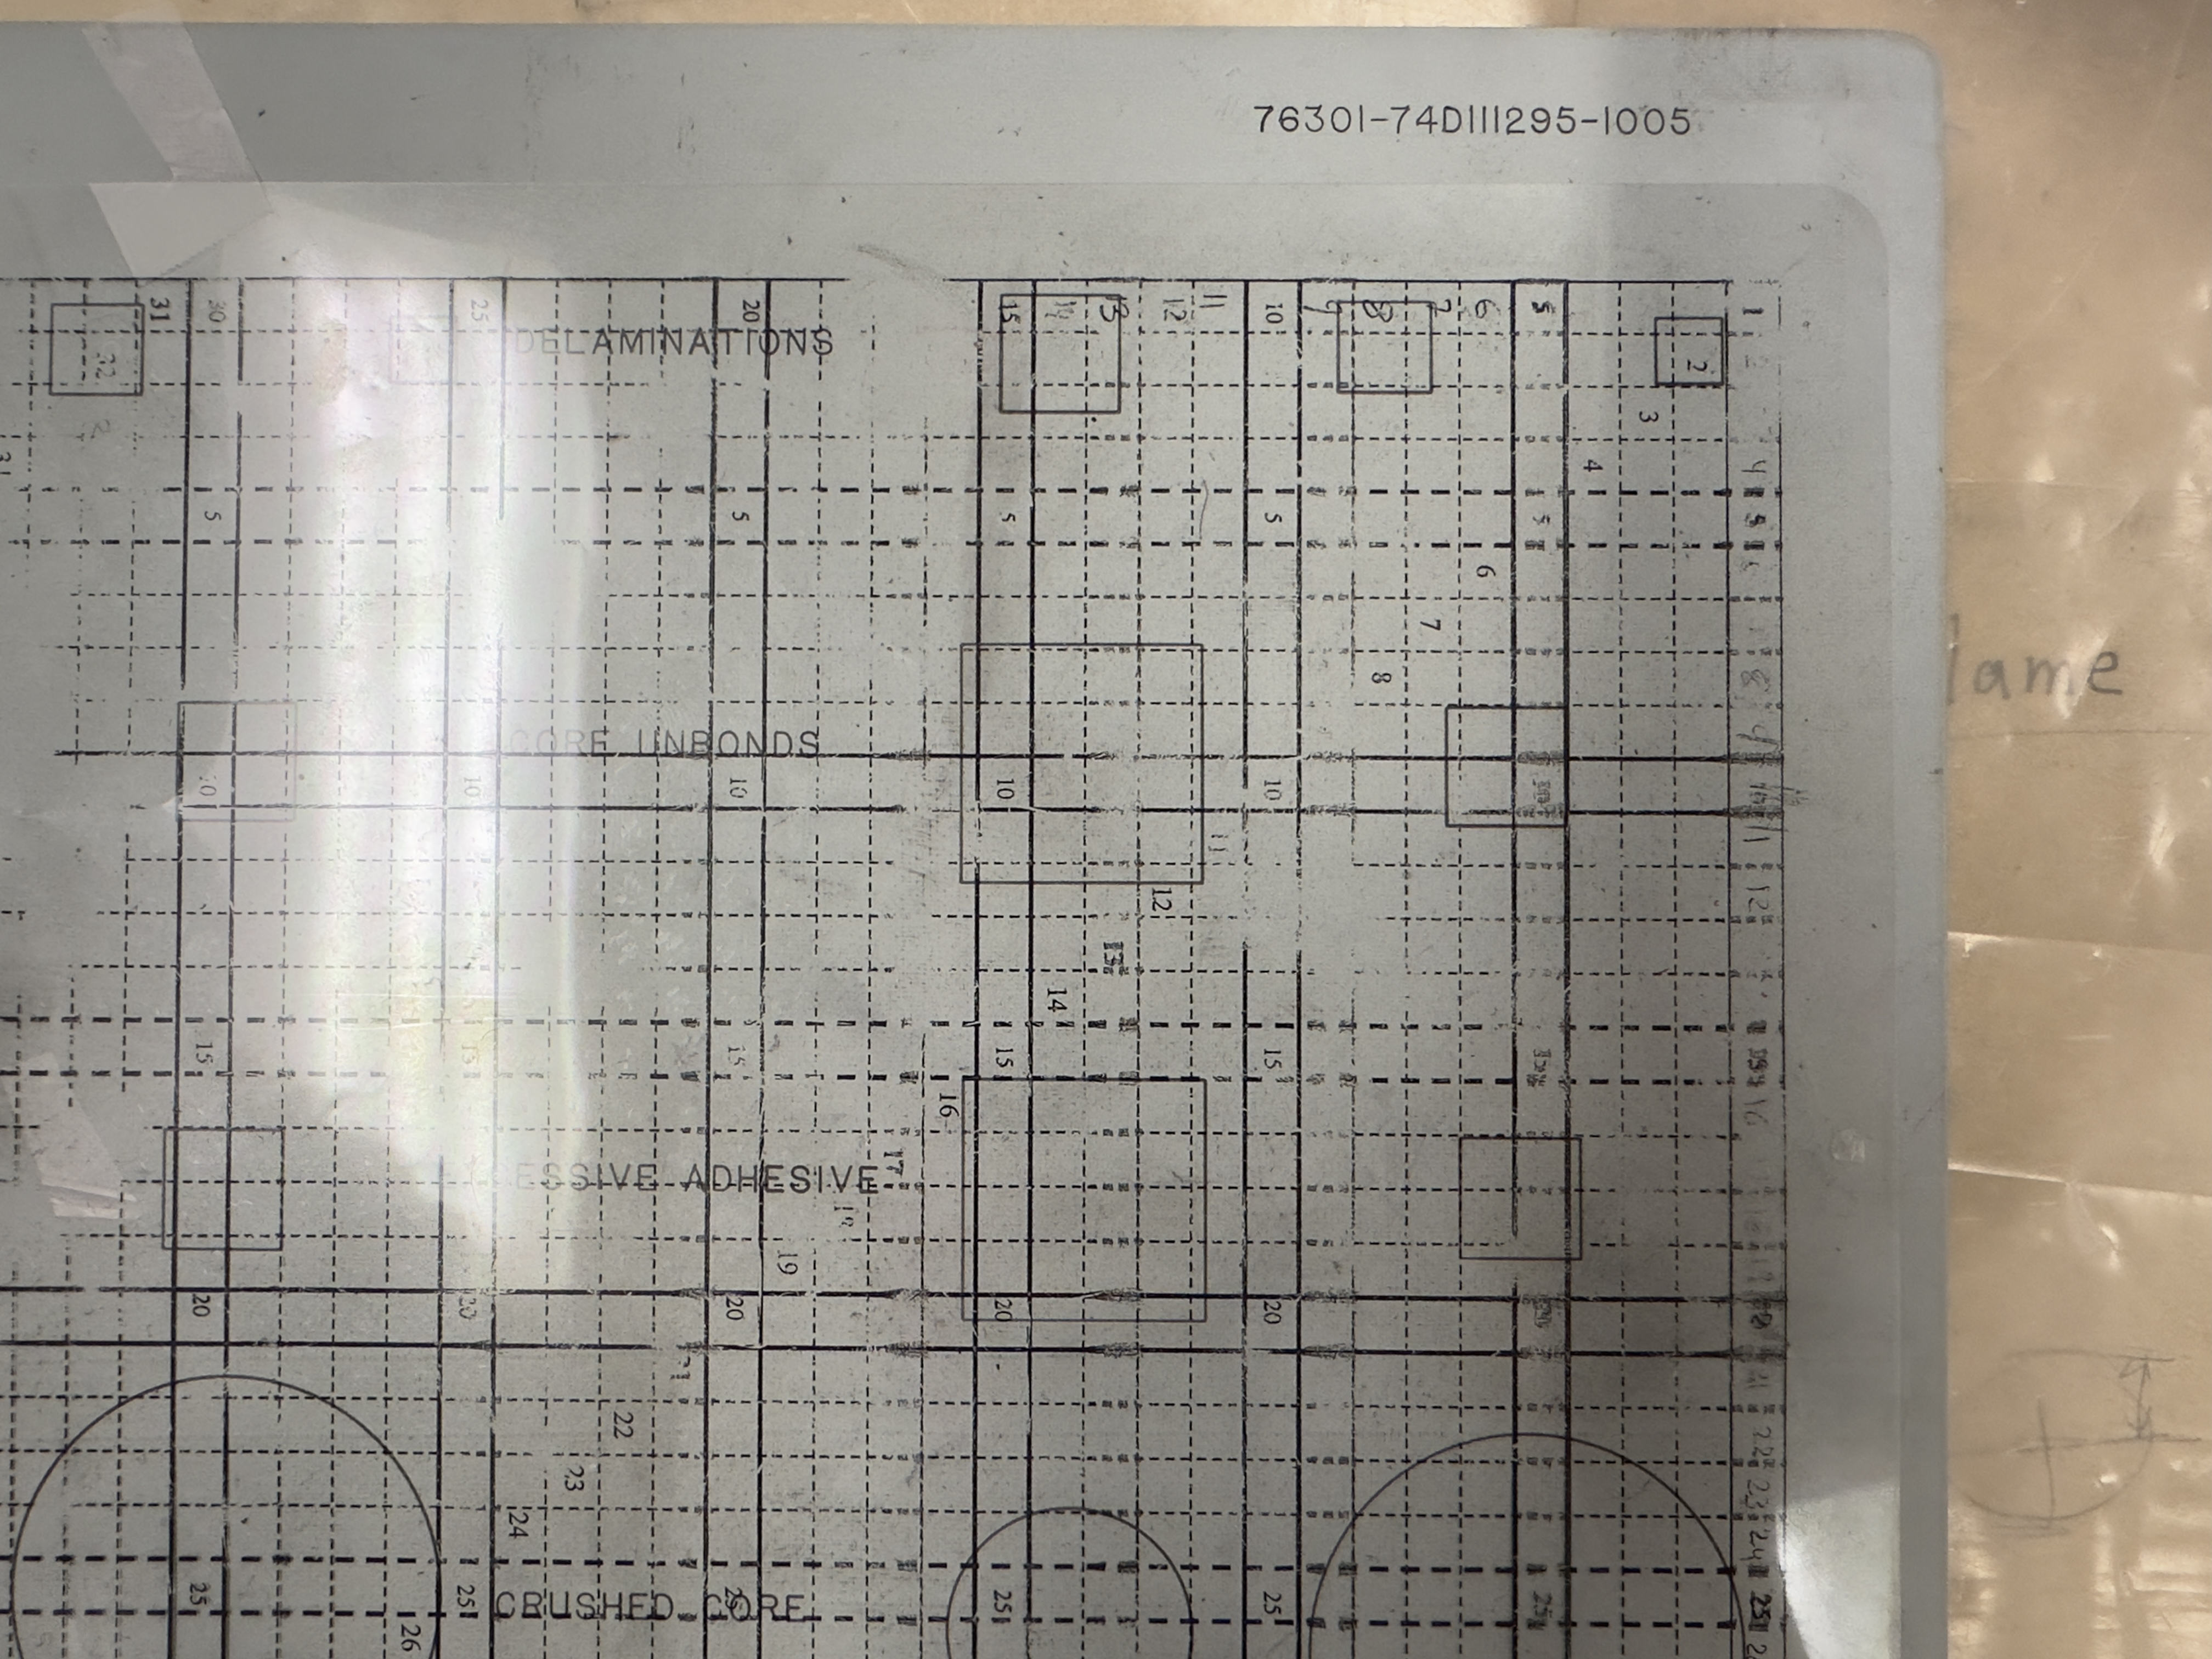
\includegraphics[width=4in]{images/graphs/tap testing/S4G2tap1-orientation}
	\caption{Orientation of the clear grid on the honeycomb sample in the first tap test (upper half).}
	\label{fig:tt1_orientation}
\end{figure}

The results of this tap test are shown in Figures \ref{fig:tt1_grid}, \ref{fig:tt1_2d}, and \ref{fig:tt1_3d}.

\begin{figure}[htbp]
	\centering
	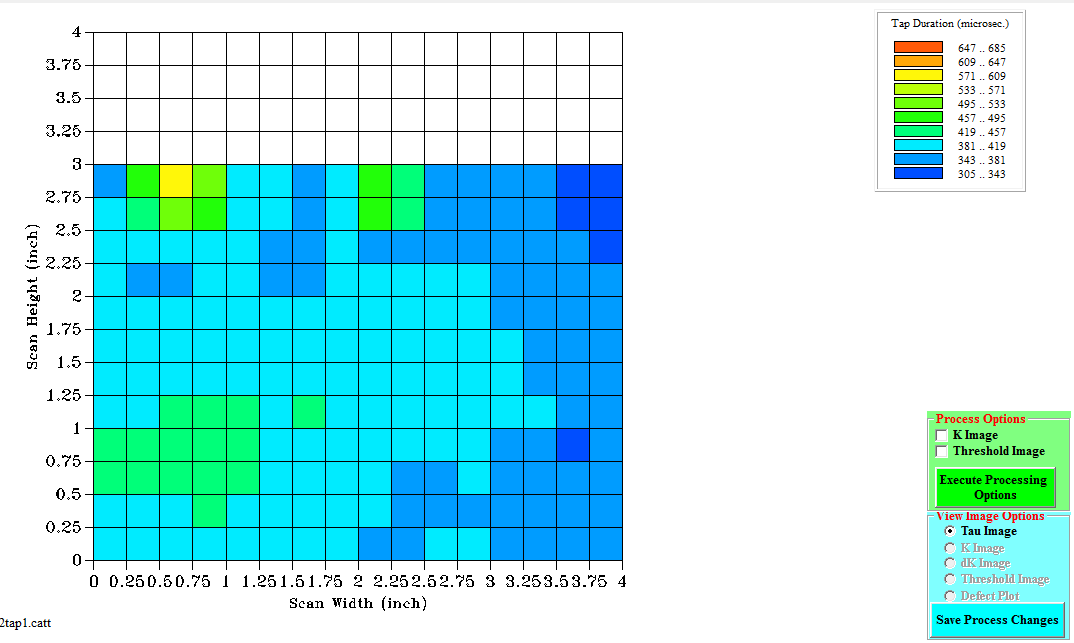
\includegraphics[width=4in]{images/graphs/tap testing/S4G2tap1-grid}
	\caption{Grid results from the first tap test (upper half).}
	\label{fig:tt1_grid}
\end{figure}

\begin{figure}[htbp]
	\centering
	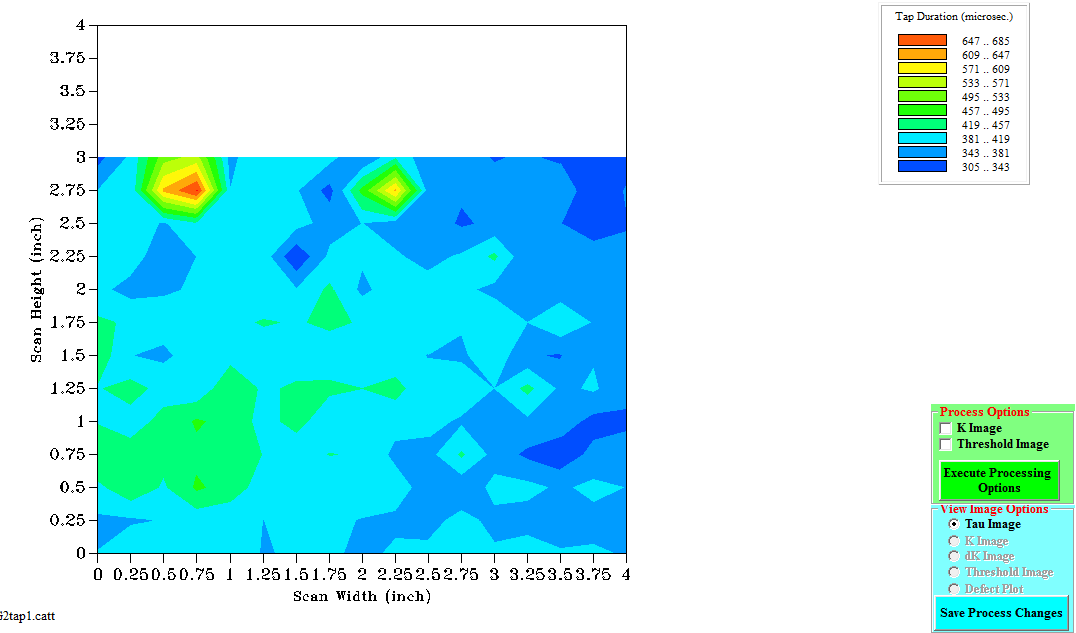
\includegraphics[width=4in]{images/graphs/tap testing/S4G2tap1-2D}
	\caption{2D visual results from the first tap test (upper half).}
	\label{fig:tt1_2d}
\end{figure}

\begin{figure}[htbp]
	\centering
	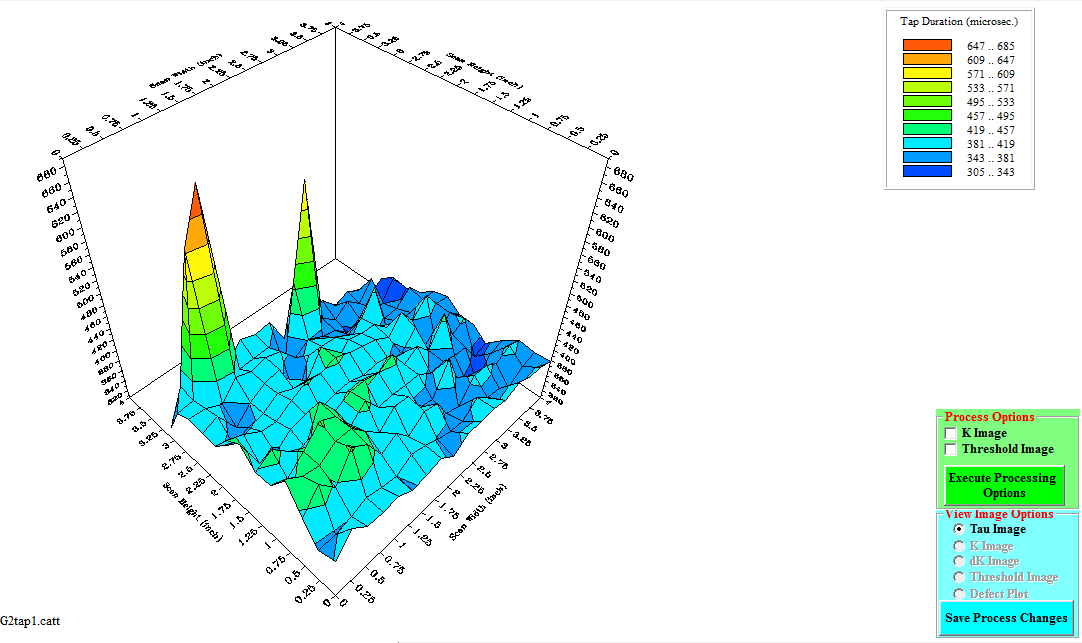
\includegraphics[width=4in]{images/graphs/tap testing/S4G2tap1-3D}
	\caption{3D visual results from the first tap test (upper half).}
	\label{fig:tt1_3d}
\end{figure}

The orientation of the clear grid and the software configuration for the second tap test run is shown in Figure \ref{fig:tt2_orientation}.

\begin{figure}[htbp]
	\centering
	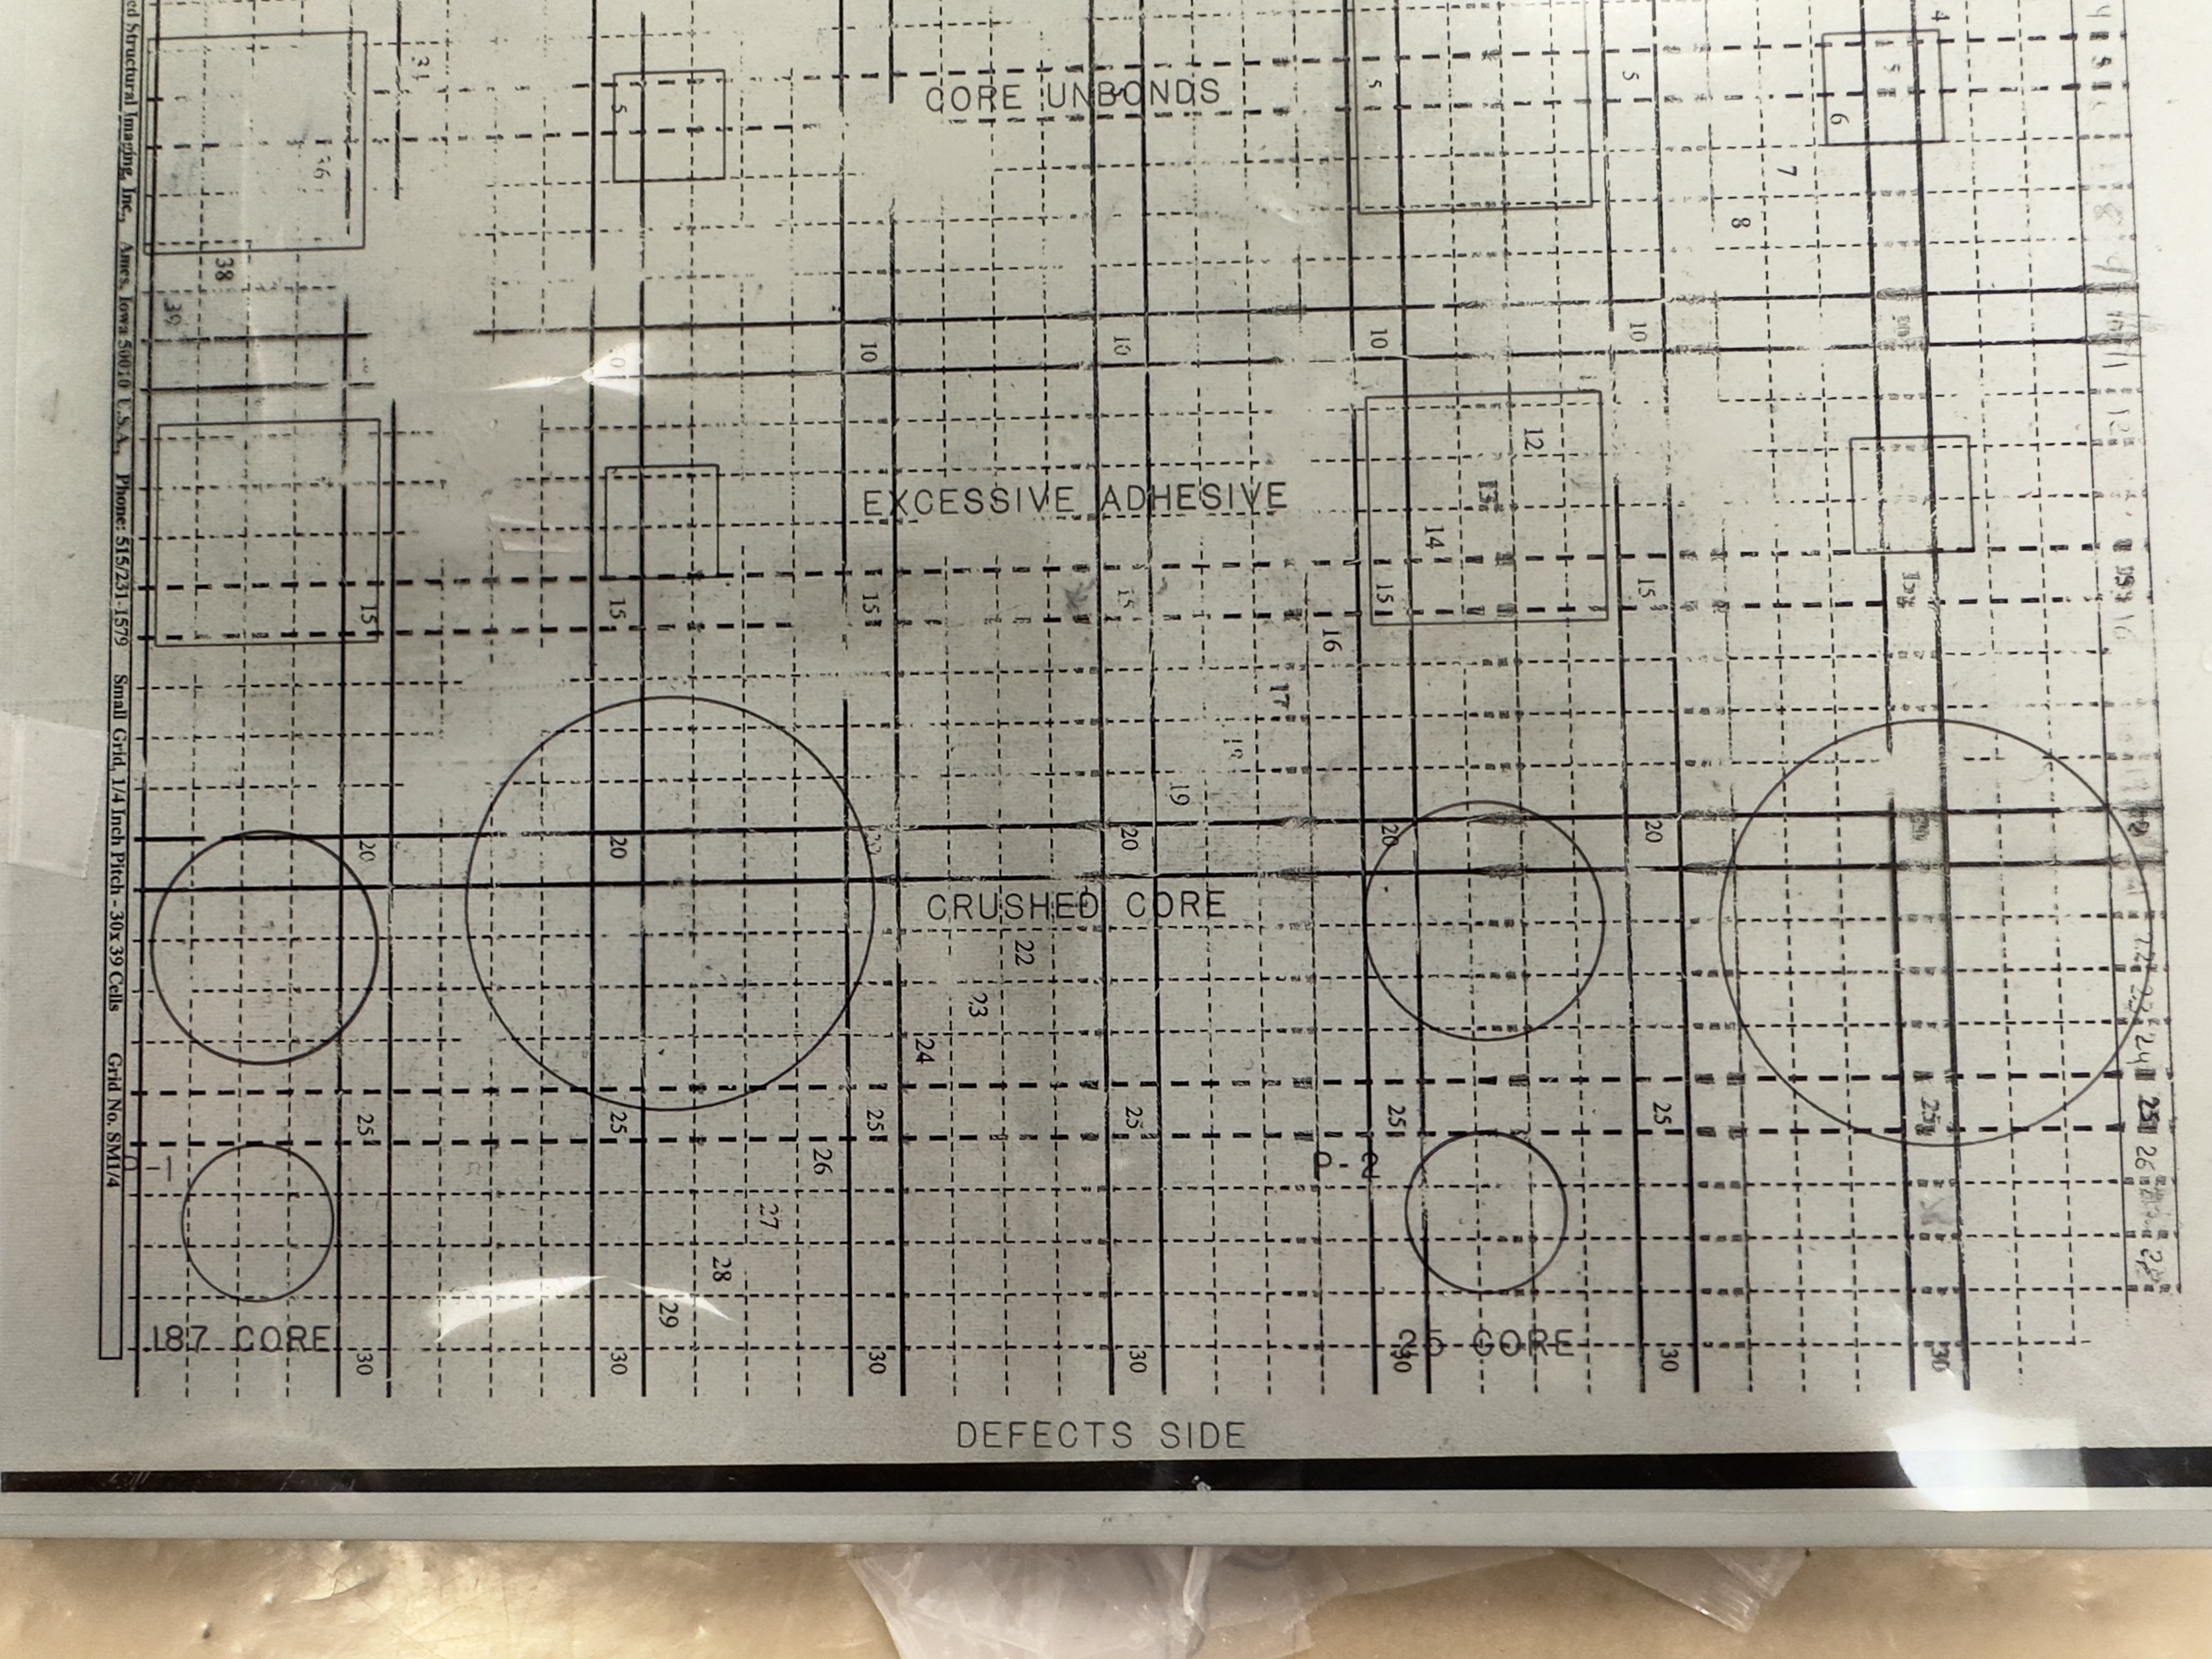
\includegraphics[width=4in]{images/graphs/tap testing/S4G2tap2-orientation}
	\caption{Orientation of the clear grid on the honeycomb sample in the second tap test (lower half).}
	\label{fig:tt2_orientation}
\end{figure}

The results of this tap test are shown in Figures \ref{fig:tt2_grid}, \ref{fig:tt2_2d}, and \ref{fig:tt2_3d}.

\begin{figure}[htbp]
	\centering
	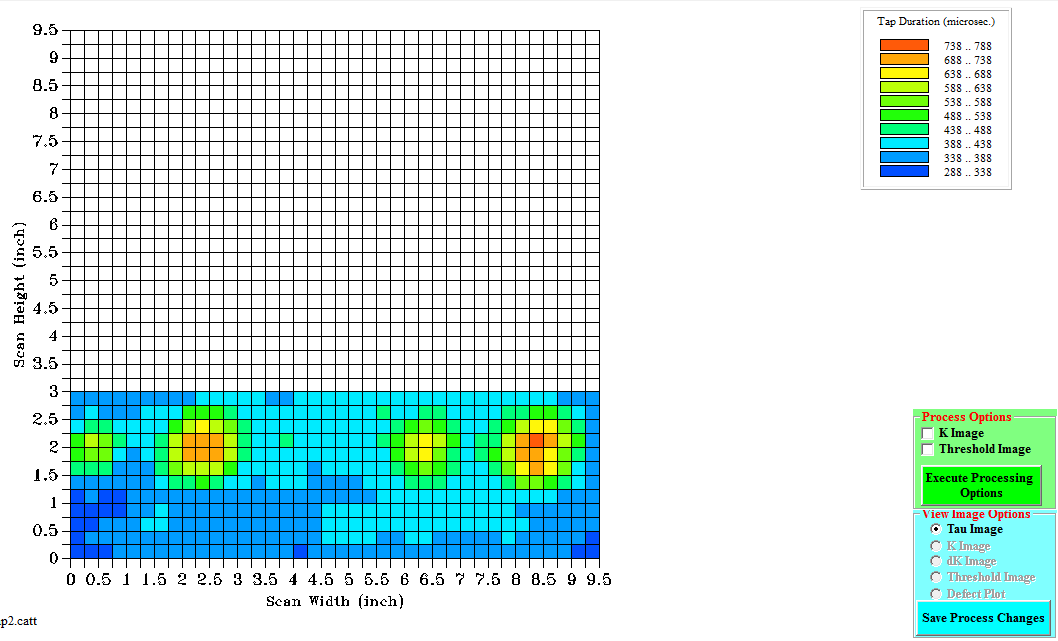
\includegraphics[width=4in]{images/graphs/tap testing/S4G2tap2-grid}
	\caption{Grid results from the second tap test (lower half).}
	\label{fig:tt2_grid}
\end{figure}

\begin{figure}[htbp]
	\centering
	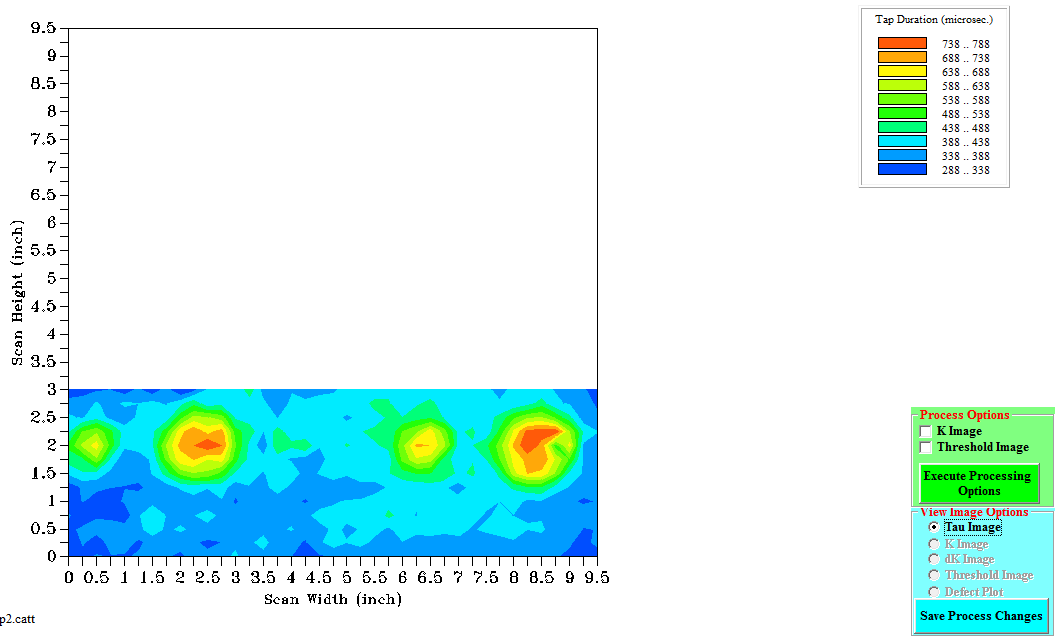
\includegraphics[width=4in]{images/graphs/tap testing/S4G2tap2-2D}
	\caption{2D visual results from the second tap test (lower half).}
	\label{fig:tt2_2d}
\end{figure}

\begin{figure}[htbp]
	\centering
	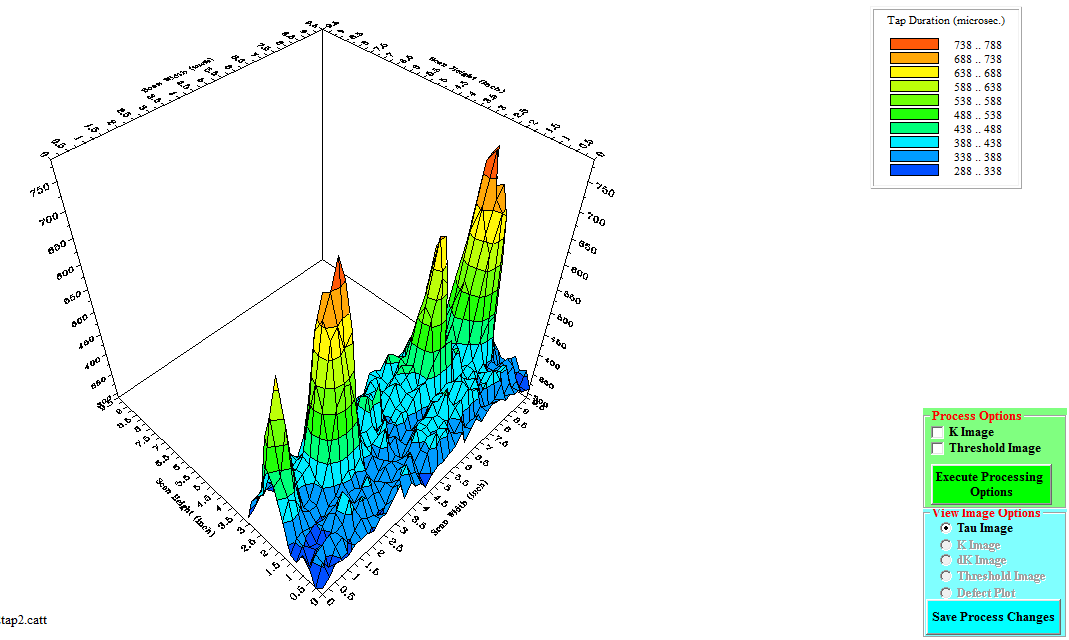
\includegraphics[width=4in]{images/graphs/tap testing/S4G2tap2-3D}
	\caption{3D visual results from the second tap test (lower half).}
	\label{fig:tt2_3d}
\end{figure}

\chapter{Conclusion} \label{conclusion-chapter}
\section{Analysis} \label{analysis}
\subsection{Tap Testing} \label{tap_testing}
% TODO: Revise
% TODO: FIX FIGURE REFERENCES
\textbf{Question 1}

Areas with delamination and core unbonds were tested in tap test \num{1}; the crushed core was tested in tap test \num{2}. As seen in Figure <INSERT FIG REFERENCE> above, delamination was much easier to detect than core unbonds. There is a clear detection of the first two defect areas in the delamination zone, but the third was undetectable. In the defect areas where there were core unbonds, there is a slight section where the tap duration was somewhere between \qtyrange{415}{495}{\micro\second}. This is especially seen in the largest defect area, but as the test continued, the smallest defect area was completely undetectable. Moving to tap test two, the defect areas where much more detectible. Starting from the left defect region, the two largest defect areas were extremely noticeable. It is clear to see that the medium sized defect had a largest duration of \qtyrange{638}{688}{\micro\second}, and the largest area had a duration of \qtyrange{738}{788}{\micro\second}. Moving to the right side of the defect area, all three defects were detected. The smallest had a barely noticeable defect, but was still present with a duration of \qtyrange{438}{488}{\micro\second}. The other two defect areas had a duration of \qtyrange{738}{788}{\micro\second}. This shows that the defects in the .187 area were much more difficult to detect than that of the defects in the .25 defect area. Alongside this, delamination was easier to detect than the core unbonds. Overall, the crushed core was the easiest to detect of all three defects.

\textbf{Question 2}

Even with the \qty{0.25}{in} spacing, the smaller defects were difficult to detect especially in the tap tests with unbonds and delaminations. As seen in Figures <INSERT FIG REFERENCE> and <INSERT FIG REFERENCE>, the smaller defects were either completely undetectable or were extremely difficult to detect. If the tap spacing increased to \qty{0.5}{in}, our group suspects that this would have a profound effect on the ability to detect defects. As the smaller defects were barely detectable at \qty{0.25}{in} spacing, the medium sized defects would look similar to the small defects if the spacing was increased to \qty{0.5}{in}. 

\textbf{Question 3}

Delaminations were more detectable due to the surface being tapped and not attached to the core. The top skin being disconnected allows for there to be more ``give'' when being tapped. With the top skin flexing more, there is a longer contact time between the surface of the plate and the hand tap cable. The unbonded core will be a less detectable defect than the delamination. This is due to the bottom surface of the plate not being directly impacted by the hand-held cable. The table supports the bottom of the plate, and there will be little ``give,'' making the defects harder to detect.

\subsection{Eddy Current Testing} \label{eddy_current_testing}
% TODO: Revise
\textbf{Question 4}

One possible reason for lift off calibration is to ensure the phase angle is set correctly. In the lab we were told to lift the probe off of the surface if the part, then set it back down to adjust the phase angle. The phase angle was changed in each testing scenario to get the lift off trace to align with the left branch of the resistance axis.

\textbf{Question 5}

We adjusted the frequency to be higher to detect hidden cracks on the face with the cracks, but decreased it when testing the back side of the sample. As the frequency increases, the depth of penetration decreases. This makes finding the cracks on the surface much easier due to the fact the equipment is more sensitive to shallow defects. For testing the defects on the back side of the sample, we decreased the frequency to have the equipment be more sensitive to defects deeper in the sample.

\subsection{Ultrasonic Testing} \label{ultrasonic_testing}
\textbf{Question 6}

Yes, a water path distance of \qty{4.5}{in} is indeed accurate enough given the configuration of the ultrasonic test. In our experiment, we calculated the optimal water path given the focal length. We began by referring to Equation \ref{eqn:focal_law} from the AER E \num{322} lecture notes \cite{lecture_notes}.
\begin{align}\label{eqn:focal_law}
	F&=Z_1+\frac{\nu_2}{\nu_1}Z_2
\end{align}
where $F$ is the focal distance, $Z_1$ is the water path, $Z_2$ is the thickness of the specimen, $\nu_1$ is the wave speed through medium one (water), and $\nu_2$ is the wave speed through medium two (metal). To calculate the optimal water path, we arrange the equation as shown in Equation \ref{eqn:water_path}.
\begin{align}\label{eqn:water_path}
	Z_1&=F-\frac{\nu_2}{\nu_1}Z_2
\end{align}
Substituting in values, we find
\begin{align*}
	Z_1&=\qty{8}{in}-\frac{\qty{0.58}{\cm\per\micro\second}}{\qty{0.148}{\cm\per\micro\second}}\cdot\qty{23}{\mm}\cdot\frac{\qty{1}{in}}{\qty{25.4}{\mm}}\\
	&=\qty{4.45}{in}\text{ or }\qty{113.1}{\mm}
\end{align*}
Therefore, the optimal water path is \qty{4.45}{in} or \qty{113.1}{\mm}. This is approximately equal to a water path of \qty{4.5}{in} as stated in the problem statement. If we use \qty{4.5}{in} as the water path, we find that the optimal focal length is
\begin{align*}
	F&=Z_1+\frac{\nu_2}{\nu_1}Z_2\\
	&=\qty{4.5}{in}+\frac{0.58}{0.148}\cdot\qty{23}{\mm}\cdot\frac{\qty{1}{in}}{\qty{25.4}{\mm}}\\
	&=\qty{8.049}{in}
\end{align*}
Using a water path of \qty{4.5}{in} yields an optimal focal length with \qty{0.61}{\percent} variation from the actual optimal focal length of \qty{8}{in}. This is plenty of accuracy for the needs of this lab.

\textbf{Question 7}

We speculate the reason the zero-to-zero amplitude profile grossly overestimates the size of the flaw is due to how the waves interact at the edge of the flaws. When the waves are bouncing completely off the flaw, the amplitude of the wave bouncing off the flaw are at the peak amplitude. However, as the transducer is moved around the flaw, only part of the waves are bouncing back from the flaw (the other part continuing on to the bottom edge of the sample). This partial reflection reduces the amplitude. But the amplitude of the flaw reflection doesn't reach zero until the entirety of the transducer pulses are clear of the flaw.

In other words, even if a very small part of the transducer waves are reflecting off the flaw, there will be a non-zero amplitude indicating a flaw. This is demonstrated in Figure \ref{fig:flaw_detection}.

\begin{figure}[htbp]
	\centering
	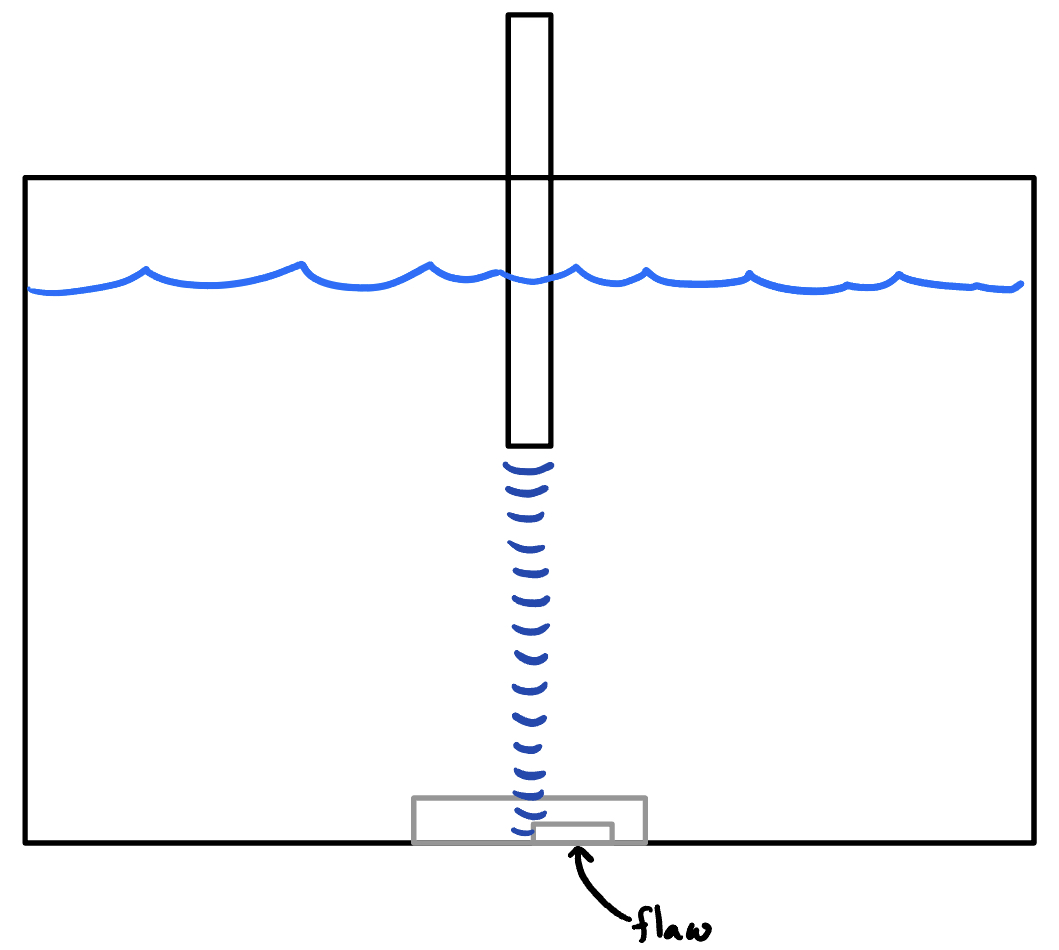
\includegraphics[width=4in]{images/flaw_detection_sketch}
	\caption{A sketch of the transducer waves reflecting on only part of the flaw.}
	\label{fig:flaw_detection}
\end{figure}

Because the flaw still shows up on the oscilloscope well after the center of the transducer has cleared the flaw, if you calculate the size of the flaw, you would be overestimating the size of the flaw. In lab, we were told to use the \qty{50}{\percent} amplitude rule as a general guide for estimating the size.

The peak amplitude we found was \qty{3.40}{\volt}. By measuring how far in each direction we had to move to find \qty{50}{\percent} of the peak amplitude (\qty{1.70}{\volt}), we calculated the flaw diameter to be \qty{6}{\mm}, which is about \qty{20}{\percent} off the actual diameter of the flaw (\qty{5}{\mm}). Given we were approximating the cut-off points of the flaw diameter, this amount of error is acceptable.

\subsection{Ultrasonic Simulation} \label{ultrasonic_simulation}
\textbf{Question 8}

We ran seventeen different simulations to determine which variables most significantly impacted the SNR. In the end, we were unable to determine qualitatively which variables had the most impact. Based on our testing, we speculate the transducer diameter and the center frequency are the most and second-most important variables in increasing the SNR. We noticed a significant increase in the SNR when we increased the transducer diameter and another fairly significant increase when we increased the center frequency.

The other variables had mixed effects on the SNR. Changing the water path seemed to move the SNR peak to the left or right and we didn't observer the focal length having a reliably positive or negative effect on the SNR.

We suspect the reason it was so difficult to identity which parameters most directly relate to the SNR is because they are linked. The water path and the focal length are related by the focal law shown in Equation \ref{eqn:focal_law}, so it seems logical that these parameters will affect the SNR independently of each other, \ie depending on the water path, increasing or decreasing the water path may increase or decrease the SNR.

\subsection{NDE and Design} \label{nde_and_design}
% TOOD: Revise
\textbf{Question 9}

Eddy current testing with a decreased frequency is the best option for this testing scenario. Eddy current testing is the best option for testing these cracks, where this is due to the ability to test the tank from the outside and detect a crack on the inside of the tank. A decreased frequency is best due to the fact that it is more sensitive to ``deeper'' defects. Eddy current testing would be perfect for this scenario due to these factors. This was demonstrated while testing the backside of BKI and BKII samples in the lab. Tap testing finds defects like delamination, core un-bonds, and crushed cores more effectively. This means that tap testing would be useless for finding cracks propagating inside a tank. Ultrasonic testing also would not work solely since the tested tank is sealed on all sides. While the tank may be full of a medium perfect for ultrasonic testing, it is impossible.

\section{Conclusion} \label{conclusion-section}
% TODO: Revise
Overall, our group gained valuable insight into which types of non-destructive testing were best for each given scenario. We struggled with aspects of the lab, such as the simulated ultrasonic testing, because we initially changed too many variables. This caused our group to run the test \num{17} times. Seventeen tests were performed to find the best mixture of changeable values we could. Regarding eddy current testing, our group could easily see the difference between each type of metal we were tasked to sort. While we could not say exactly what each metal was, there was a clear difference between all samples, with one having a noticeably larger trace than all the others. The BKI and BKII samples also provided valuable insight into how eddy current testing can be used to test for cracks on both the front side and backside of a part. Our group determined that the best way to test for the cracks inside a waste storage tank was to use eddy current testing because ultrasonic testing requires submerging the transducer face. Tap testing was ruled out as well due to the inability of tap testing to detect cracks. Tap testing is best used for layered composites or materials, making it practically useless. Ultimately, we determined eddy current testing to be the best form of non-destructive testing for this scenario because of its ability to detect cracks on the backside of a material and to test for defects on the outside of the material. Much valuable information was learned from tap testing as well. While performing testing, we did not know exactly what each defect type meant, but we could see how each defect resulted in vastly different tap durations. The crushed core had the largest tap duration, and we could detect many more defect areas than the unbonded and delamination defect areas. After learning what each defect meant, it was clear why our data appeared as is.

\printbibliography[heading=subbibintoc]
\appendix
\chapter{Code} \label{apdx:code}
\begin{verbatim}
% AER E 322 Lab 9 Spring 2023
% Section 4 Group 2
clear,clc,close all;

u = symunit;
F = 8*u.in; % [in]
V_s = 0.58*u.cm/u.us; % [cm/us]
V_w = 0.148*u.cm/u.us; % [cm/us]
T = 23*u.mm; % [mm]

L_1 = unitConvert(F - V_s / V_w * T, u.mm); % [mm]
delta_t_top = 2 * L_1 / unitConvert(V_w, u.mm); % [us]
delta_t_bot = 2 * unitConvert(T, u.cm) / V_s; % [us]

delta_t = delta_t_top + delta_t_bot; % [us]

fprintf("L_1 = %g [mm]\n" + ...
    "delta_t_top = %g [us]\n" + ...
    "delta_t_bot = %g [us]\n" + ...
    "delta_t_top + delta_t_bot = %g [us]\n", ...
    [double(separateUnits(L_1)), double(separateUnits(delta_t_top)), ...
    double(separateUnits(delta_t_bot))], double(separateUnits(delta_t)));
\end{verbatim}

\textbf{Output:}

\begin{verbatim}
L_1 = 113.065 [mm]
delta_t_top = 152.79 [us]
delta_t_bot = 7.93103 [us]
delta_t_top + delta_t_bot = 160.721 [us]
\end{verbatim}
\end{document}
